\chapter[Técnicas de TA]{Técnicas de traducción automática} \label{se:TdTA} 

\com{Aquí faltaría hablar, en algún lugar, de la relación entre las arquitecturas de traducción automática y el \emph{principio de composicionalitat}: trabajo para Mikel, que ya tiene cosas escritas. También habría que hablar (aquí o en el tema de ambigüedad) de la imposibilidad de programar el conocimiento intuitivo de los profesionales de la traducción (creencias, expectativas) para deshacer la ambigüedad, generar texto. etc. y de la necesidad de formular reglas y métodos para automatizar el proceso. Tengo notas abundantes y textos sobre esto; el problema es donde los colocamos sin rehacer completamente el tema.} 

\com{Creo que se podría explicar el modelo cero y colocar la traducción \emph{directa} como un caso típico de traducción indirecta \emph{ad hoc}} 

Este capítulo describe las técnicas o, dicho de otro modo, las estrategias básicas usadas por los programas de traducción automática. 

Hay dos grandes grupos de sistemas de traducción automática: \begin{itemize} \item Por un lado, los sistemas de traducción automática \textbf{basados en reglas} (en inglés, \emph{rule-based machine translation}) o \textbf{basados en conocimiento} (en inglés \emph{knowledge-based machine translation}). En estos sistemas, la información necesaria para realizar la traducción automática (diccionarios, reglas) la han escrito personas expertas de manera \emph{deductiva}: es decir, han pensado en como automatizar el proceso de traducción automática y  han deducido la información necesaria para realizarla. Entre estos sistemas, podemos distinguir: \begin{itemize} \item Los sistemas de traducción automática \emph{indirecta por transferencia} (apartado~\ref{ss:classtrans}), entre los cuales, podemos distinguir, de acuerdo con el nivel de abstracción lingüística: \begin{itemize} \item los sistemas de transferencia morfológica avanzada (a veces denominados de ``traducción directa'', a pesar de que no lo son; apartado~\ref{s3:STMorf}); \item los sistemas de transferencia sintáctica (apartado~\ref{s3:transyn}), y los \item sistemas de transferencia semántica (apartado~\ref{s3:transsem}). \end{itemize} \item Los sistemas de traducción automática \emph{por interlingua} (apartado~\ref{ss:interlingua}). \end{itemize} \item Por otro lado, los sistemas de traducción automática \textbf{basados en corpus} (en inglés \emph{corpus-based machine translation}). En estos sistemas (véase el apartado~\ref{ss:induc}), la información necesaria para realizar la traducción automática se \emph{aprende} automáticamente de manera \emph{inductiva} a partir de un \emph{corpus} paralelo, es decir, de grandes cantidades de textos y sus traducciones, previamente \emph{segmentados} y \emph{alineados} para poner cada oración de un texto en correspondencia con su traducción en el otro.\footnote{Los textos del corpus de aprendizaje pueden además ser anotados o procesados con algún tipo de procesador lingüístico como por ejemplo un analizador morfológico o sintáctico.} Los sistemas basados en corpus más comunes son los de \emph{traducción automática estadística}, en los que lo que se aprende son modelos probabilísticos de traducción. Durante el decenio de 2010 se está investigando en sistemas que usan el llamado \emph{aprendizaje profundo} (en inglés \emph{deep learning}) basado en \emph{redes neurals artificiales}, las cuales se basan vagamente en cómo funciona el cerebro humano. \end{itemize} 

%\section{La traducció automàtica basada en regles, entre el principi
%  de composicionalitat semàntica i la traducció mot per mot}
\section{Funcionamiento de la traducción automática} \label{se:aprox} 

Los sistemas de traducción automática \emph{reales}, es decir, los que se usan en la realidad, son el resultado de hacer una serie de aproximaciones sobre la traducción automática \emph{ideal} para hacer el problema de la traducción computacionalmente abordable. 

La mayoría de los sistemas de traducción automática, independientemente de si son basados en reglas o en corpus, adoptan la que podrían denominar \textbf{aproximación oracional}, según la cual \emph{traducir textos es traducir oraciones}. Esta aproximación excluye el tratamiento de algunos aspectos de la estructura del discurso. 

Una vez hecha esta aproximación general, el resto de aproximaciones dependen del tipo de sistema de traducción automática. La mayoría de los sistemas de traducción automática basados en conocimiento abordan la traducción como la aplicación del \emph{principio de composicionalidad semántica} (PCS, capítulo~\ref{se:ambig}), el cual afirma que la interpretación (el significado) de una oración se construye composicionalment a partir de las interpretaciones de las palabras, siguiendo los agrupamientos dictados por su árbol de análisis sintáctico, y también a la inversa, que las oraciones se pueden construir composicionalmente a partir de las interpretaciones \citep{tellier00p}. Traducir una oración, en este esquema, compuerta: \begin{itemize} \item hacer el análisis sintáctico completo, \item asignar interpretación a cada palabra, \item construir composicionalment una interpretación de la oración, \item analizarla para obtener palabras y un árbol de análisis sintáctico para la lengua meta (LM), y generar \item una oración en LM a partir de las palabras y el árbol. \end{itemize} Este es básicamente el \emph{modus operandi} de los sistemas de \emph{interlingua} (que se discutirán en la sección~\ref{ss:interlingua}) y constituye la \textbf{aproximación composicional}. No olvidemos que esta descripción asume que la ambigüedad léxica (múltiples interpretaciones de las palabras) y estructural (más de un árbol de análisis sintáctico) ha sido idealmente resuelta. 

Por otro lado, los sistemas de traducción automática indirecta por transferencia (que se discutirán en el apartado \ref{ss:classtrans}) son el resultado de una serie de aproximaciones (muchas de ellas inevitables) sobre un modelo ideal y teóricamente motivado basado en el \emph{principio de composicionalidad semántica}. Estos sistemas también se pueden ver como el resultado de una serie de refinamientos inevitables sobre un sistema de traducción \emph{palabra por palabra} (veáis el apartado~\ref{ss:dirindir}), es decir, como una serie de operaciones adicionales que se tienen que hacer además de ir sustituyendo cada palabra por un equivalente constante. Por ejemplo, para producir traducciones aceptables, rápidas e inteligibles, incluso entre lenguas muy parecidas, se debe añadir un procesamiento léxico robusto (por ejemplo, para tratar expresiones multipalabra o para elegir equivalentes adecuados para palabras léxicamente ambiguas) y un procesamiento estructural local o global que se basa en reglas simples y bien formuladas para algunas transformaciones estructurales (reordenamientos, concordancia, etc.). 

% Aquests refinaments impliquen necessàriament un cert nivell
% d'anàlisi del text original, el qual produeix una representació
% intermèdia, abstracta, d'aquest: el sistema de traducció automàtica
% esdevé \emph{indirecte}, com ara els sistemes de transferència
% discutits amb més detall més avall (apartat~\ref{ss:classtrans}).
Cómo en el caso de los traductores profesionales, los sistemas de traducción automática no siempre necesitan \emph{comprender} las frases en lengua origen (LO) , es decir, construir una interpretación explícita. Esta noción, que puede parecer polémica, no lo es tanto: quién traduce como profesional un manual de mecánica del automóvil o un texto de física teórica lo puede hacer sin tener que entender completamente las disciplinas correspondientes. Los sistemas de \emph{transferencia} sintáctica (veáis el apartado \ref{s3:transyn}) toman un atajo y van directamente del árbol de análisis sintáctico y las palabras en LO al árbol y las palabras en LM. Lo hacen aplicando transformaciones al árbol de análisis sintáctico (\emph{transferencia estructural}) y sustituyendo las palabras (\emph{transferencia léxica}), sin construir una representación explícita de la interpretación; esta es la \textbf{aproximación de transferencia}. Dependiendo del tipo concreto de sistema de traducción automática por transferencia, todavía son posibles más aproximaciones, como veremos más abajo. 

% \item[Aproximació núm.\ 3:] Quan les llengües involucrades són
%   sintàcticament similars (per exemple, quan estan emparentades),
%   no es fa l'anàlisi sintàctica completa: la transferència lèxica
%   és completa però la transferència estructural és parcial i local
%   i només es fa on és necessària.  Aquesta aproximació és
%   l'aproximació de la \emph{transferència parcial}. Els sistemes
%   anomenats \emph{transformers} o també de transferència
%   morfològica
%   avançada (vegeu~\ref{s3:STMorf}) \citep[4.2]{arnold94b}, molts
%   dels quals estan disponibles per Internet,\footnote{Per exemple,
%   SDL Transcend està disponible en
%   \url{http://www.freetranslation.com} i Reverso, en
%   \url{http://www.reverso.net}.} són exemples d'aquesta
%   aproximació.
Por último, los sistemas de traducción automática estadística (que se discutirán en el apartado \ref{ss:induc}) hacen \textbf{asunciones de independencia estadística} para poder modelar estadísticamente el proceso de traducción. Por ejemplo, el \emph{modelo de traducción}, que se usa para estimar la probabilidad de que un segmento de texto en LM sea la traducción de un segmento de texto en LO, asume que la traducción de un segmento es independiente de la traducción del resto de segmentos de la oración; es decir, asume que no hay que tener en cuenta el contexto para traducir cada uno de los segmentos de la oración en LO. 

\section{Traducción directa y traducción indirecta} \label{ss:dirindir} Las estrategias de traducción automática se pueden dividir en dos grandes grupos, las \emph{directas} y las \emph{indirectas}. La estrategia \emph{directa} se denomina así porque la traducción de una frase se produce directamente, sin que se genere una representación intermedia de la frase; a veces también se suele denominar vagamente traducción \emph{palabra por palabra}. La estrategia \emph{indirecta} produce, a partir de la frase en LO, una representación intermedia de la frase que después se usa para traducirla. Veremos más adelante de qué naturaleza son estas representaciones intermedias. 

\label{pg:mpm} Una formalización posible de la traducción automática directa más sencilla posible es la traducción \emph{palabra a palabra}: el sistema lee el texto original palabra a palabra de izquierda a derecha,\footnote{Se asume que el texto está ya segmentado en palabras, operación que puede no ser trivial en algunos idiomas como por ejemplo el japonés o el chino, que no usan espacios en blanco para separar las palabras.} sustituye cada palabra original por un equivalente fijo (de una palabra, de más palabras, o incluso de cero palabras) en LM sin tener en cuenta el contexto y escribe las palabras uno a uno y en el mismo orden en el texto meta. Por ejemplo, si la frase tiene \(N\) palabras, \begin{displaymath} m_1\; m_2\; m_3\; \cdots \;m_N \end{displaymath} la traducción \emph{palabra por palabra} es \begin{displaymath} T(m_1)\; T(m_2)\; T(m_3)\; \cdots\; T(m_N) \end{displaymath} donde \(T(m)\) representa el equivalente fijo de la palabra \(m\) en la LM, que puede tener cero, uno o más palabras. Por ejemplo, la traducción \emph{palabra por palabra} al inglés de la frase catalana \emph{Este ejercicio práctico es muy sencillo}, con \(m_1=\mbox{\emph{Este}}\), \(m_2=\mbox{\emph{ejercicio}}\), etc., podría ser \emph{This exercise practical it is very simple} (incorrecta), donde, por ejemplo, \(T(m_4)=T(\mbox{\emph{es}})=\mbox{\emph{it is}}\). 

Ningún sistema real de traducción automática usa este modelo tan rudimentario de traducción, puesto que es incapaz de producir traducciones automáticas útiles, ni siquiera para lenguas muy similares: todos los sistemas van más allá y realizan operaciones adicionales. Por eso mismo, el modelo \emph{palabra a palabra} se puede usar como modelo de referencia o \emph{modelo cero} a la hora de estudiar que más hacen los sistemas existentes, o que más hay que hacer para producir traducciones automáticas útiles para un par de lenguas. 

% Una aproximació a la traducció humana assistida per ordinador (és a
% dir, semiautomàtica) que es pot veure com un tipus de traducció
% directa ---que usa segments de text més llargs com ara les oracions
% en compte dels mots--- és la que s'usa en les anomenades
% \emph{memòries de traducció} (vegeu el capítol~\ref{se:memtrad}).
\section{Traducción indirecta por transferencia} \label{ss:classtrans} 

Muchos de los sistemas indirectos basados en reglas son sistemas de \emph{transferencia}. Un \emph{sistema de traducción automática indirecta por transferencia}, o, abreviadament, \emph{sistema de transferencia} es el que hace las traducciones en tres fases muy diferenciadas llamadas \emph{análisis}, \emph{transferencia} y \emph{generación}; cada una de estas fases es realizada por un módulo (un subprograma) del sistema: \begin{itemize} \item El módulo de \emph{análisis} es un módulo monolingüe que produce, a partir de la frase en LO, una \emph{representación abstracta del texto origen} (RATO). En la RATO se eliminan todos los detalles de la frase en LO que no se consideran relevantes para la traducción y se destacan aquellas características y relaciones que sí que lo son. Por ejemplo, podría convenir que las frases inglesas ``Sam gave a book to Leslie'' y ``Sam gave Leslie a book'' \citep{arnold93j} tuvieron la misma RATO. \item El módulo de \emph{transferencia} es un módulo bilingüe que lee la RATO y genera otra representación abstracta similar, pero para la LM, la \emph{representación abstracta del texto meta} (RATM). \item El módulo de \emph{generación} (o, menos comúnmente, \emph{síntesis}) genera a partir de la RATM un texto \emph{concreto}: la traducción en bruto. \end{itemize} Estas tres fases se esquematizan en la figura~\ref{fg:transfer}. 

\begin{figure} \begin{center} \parbox{0.5cm}{TO} $\to$ \framebox{\parbox{0.2cm}{A}} $\to$ \parbox{1.0cm}{RATO} $\to$ \framebox{\parbox{0.2cm}{T}} $\to$ \parbox{1.25cm}{RATM} $\to$ \framebox{\parbox{0.25cm}{G}} $\to$ \parbox{0.5cm}{TM} \end{center} \caption{Fases de análisis (A), transferencia (T) y generación (G) en un sistema de traducción indirecta por transferencia (TO = texto origen; RATO = representación abstracta del texto origen; RATM = representación abstracta del texto meta; TM = texto meta).} \label{fg:transfer} \end{figure} 

Las representaciones abstractas \emph{acercan} las dos lenguas eliminando algunos detalles específicos y destacando características generales que pueden así ser tratadas más fácilmente por el módulo de transferencia. Por ejemplo, los adjetivos catalanes van normalmente detrás de los sustantivos mientras que los ingleses van normalmente delante; traducir comporta, por lo tanto, cambiar los adjetivos de posición. Pero, para ello, hay que identificar qué palabras son adjetivos y sustantivos: la fase de análisis se puede encargar de esta tarea para que la fase de transferencia pueda aplicar reglas generales sin preocuparse de cuáles son los adjetivos o los sustantivos concretos. 

% \begin{figure} % figura vella
% \begin{center}
% %TexCad Options
% %\grade{\off}
% %\emlines{\off}
% %\beziermacro{\on}
% %\reduce{\on}
% %\snapping{\off}
% %\quality{2.00}
% %\graddiff{0.01}
% %\snapasp{1}
% %\zoom{1.00}
% \unitlength 1.00mm
% \linethickness{0.4pt}
% \begin{picture}(100.00,20.00)
% \put(10.00,10.00){\makebox(0,0)[cc]{text LO}}
% \put(40.00,10.00){\makebox(0,0)[cc]{RALO}}
% \put(70.00,10.00){\makebox(0,0)[cc]{RALM}}
% \put(100.00,10.00){\makebox(0,0)[cc]{text LM}}
% %\vector(20.00,10.00)(30.00,10.00)
% \put(30.00,10.00){\vector(1,0){0.2}}
% \put(20.00,10.00){\line(1,0){10.00}}
% %\end
% %\vector(50.00,10.00)(60.00,10.00)
% \put(60.00,10.00){\vector(1,0){0.2}}
% \put(50.00,10.00){\line(1,0){10.00}}
% %\end
% %\vector(80.00,10.00)(90.00,10.00)
% \put(90.00,10.00){\vector(1,0){0.2}}
% \put(80.00,10.00){\line(1,0){10.00}}
% %\end
% \put(25.00,15.00){\makebox(0,0)[cc]{anàl.}}
% \put(55.00,15.00){\makebox(0,0)[cc]{transf.}}
% \put(85.00,15.00){\makebox(0,0)[cc]{gen.}}
% \end{picture}
% \end{center}
% \caption{Fases d'anàlisi, transferència i generació en un
% sistema de traducció indirecta per transferència.}
% \label{fg:transfer} 
% \end{figure}
La arquitectura de transferencia es el modelo estándar para la traducción automática basada en reglas o conocimiento contemporánea, y lo ha sido por muchos años \citep{arnold93j}. 

Los sistemas de transferencia se clasifican según la naturaleza de las representaciones abstractas que utilizan: se puede hablar, en orden de profundidad del análisis, de sistemas de \emph{transferencia morfológica}, de \emph{transferencia sintáctica} o de {\em transferencia semántica}. La elección de la profundidad del análisis se debe fundamentar en la naturaleza y la profundidad de las divergencias de traducción \citep{vandooren93b} entre las lenguas implicadas. 

La arquitectura de transferencia tiene tres características interesantes que merecen ser mencionadas: \begin{description} \item[Funcionamiento como cadena de montaje.] El sistema de transferencia funciona como una \emph{cadena de montaje}: cómo los tres módulos trabajan de izquierda a derecha y en una única pasada, no hace falta que un módulo espere que el anterior acabo con el texto: pueden trabajar paralelamente; ello hace que los sistemas de esta naturaleza sean muy rápidos. \item[Modularitat.] La división en \emph{módulos} o etapas bien diferenciadas (análisis, transferencia y generación)  permite la reutilización. Por ejemplo, si hemos construido un sistema de transferencia que traduce del inglés al español: \begin{center} \parbox{0.5cm}{en} $\to$ \framebox{\parbox{0.5cm}{A\(_\mathrm{en}\)}} $\to$ \framebox{\parbox{1.125cm}{T\(_\mathrm{en\to es}\)}} $\to$ \framebox{\parbox{0.5cm}{G\(_\mathrm{es}\)}} $\to$ \parbox{0.5cm}{es} \end{center} podemos aprovechar el módulo de análisis del inglés  (A\(_\mathrm{en}\)) para construir un sistema del inglés al catalán: \begin{center} \parbox{0.5cm}{en} $\to$ \framebox{\parbox{0.5cm}{A\(_\mathrm{en}\)}} $\to$ \framebox{\parbox{1.125cm}{T\(_\mathrm{en\to ca}\)}} $\to$ \framebox{\parbox{0.5cm}{G\(_\mathrm{ca}\)}} $\to$ \parbox{0.5cm}{ca} \end{center} o usar el módulo de generación del español G\(_\mathrm{es}\) para construir un sistema del neerlandés al español: \begin{center} \parbox{0.5cm}{en} $\to$ \framebox{\parbox{0.5cm}{A\(_\mathrm{nl}\)}} $\to$ \framebox{\parbox{1.125cm}{T\(_\mathrm{nl\to es}\)}} $\to$ \framebox{\parbox{0.5cm}{G\(_\mathrm{es}\)}} $\to$ \parbox{0.5cm}{es} \end{center} \item[Reversibilidad parcial.] Si se separan los datos lingüísticos usados por cada uno de los tres módulos, \label{pg:separacio} es posible una \emph{reversibilidad parcial}. Si en el sistema inglés--español de arriba separamos los \emph{datos lingüísticos} de cada uno de los tres módulos del \emph{software} que procesa estos datos (dA\(_\mathrm{en}\), dT\(_\mathrm{en\to es}\), dg\(_\mathrm{es}\)) podemos definir un \emph{motor} genérico de traducción (A, T, G) que vale para cualquier par de lenguas: \begin{center} \parbox{0.5cm}{en} $\to$ \framebox{\parbox{0.75cm}{dA\(_\mathrm{en}\)\\ A}} $\to$ \framebox{\parbox{1.5cm}{dT\(_\mathrm{en\to es}\)\\ T}} $\to$ \framebox{\parbox{0.75cm}{dG\(_\mathrm{es}\)\\ G}} $\to$ \parbox{0.5cm}{es} \end{center} Si ahora queremos escribir el sistema de traducción inverso, español--inglés, es decir, \begin{center} \parbox{0.5cm}{es} $\to$ \framebox{\parbox{0.75cm}{dA\(_\mathrm{es}\)\\ A}} $\to$ \framebox{\parbox{1.5cm}{dT\(_\mathrm{es\to en}\)\\ T}} $\to$ \framebox{\parbox{0.75cm}{dG\(_\mathrm{en}\)\\ G}} $\to$ \parbox{0.5cm}{en} \end{center} podríamos sacar ventaja del hecho que hay grandes parecidos entre los datos lingüísticos de este sistema y las del sistema anterior: \begin{itemize} \item los datos que necesitamos para el análisis del español dA\(_\mathrm{es}\) son muy similares a los datos de generación del español dg\(_\mathrm{es}\) del sistema existente: para analizar el español podemos reciclar una buena parte de los datos que se usaban para generarlo en el sistema anterior; \item los datos que necesitamos para la generación del inglés dg\(_\mathrm{en}\) son muy similares a los datos de análisis del inglés dA\(_\mathrm{en}\) del sistema existente: para generar el inglés podemos reciclar una buena parte de los datos que se usaban para analizarlo en el sistema anterior; \item los datos de transferencia del español al inglés dT\(_\mathrm{es\to en}\) son muy similares a los datos de transferencia del inglés al español dT\(_\mathrm{en\to en}\) del sistema existente: para transferir de español a inglés podemos usar una buena parte de los datos que se usaban para transferir desde el inglés al español en el sistema anterior (por ejemplo, podemos ``dar la vuelta'' a los diccionarios bilingües y podríamos aprovechar muchas entradas). \end{itemize} \end{description} 

\subsection{Sistemas de transferencia morfológica avanzada} \label{s3:STMorf} 

En los sistemas de transferencia \emph{morfológica avance} ---también llamados sistemas de \emph{transferencia sintáctica parcial} o \emph{transformers} \citep[4.2]{arnold94b}--- la fase de \emph{análisis} analiza morfológicamente las palabras de la frase y los desambigua en caso de ambigüedad léxica categorial pero sólo identifica las relaciones (sintácticas) entre ellos usando patrones muy sencillos.\footnote{Algunos sistemas de transferencia morfológica avanzada disponibles en Internet son: SDL Transcend (\url{http://www.freetranslation.com}) Reverso (\url{http://www.reverso.net}), y Apertium (\url{http://www.apertium.org}).} La sección~\ref{s3:anmor} da más detalles sobre los procesos y los métodos de análisis y generación morfológicos. 

De hecho, los sistemas de transferencia morfológica avanzada se pueden ver como el resultado de hacer una tercera aproximación, añadida a las dos (\emph{aproximación oracional} y aproximación \emph{de transferencia}) discutidas en el apartado~\ref{se:aprox}: \begin{quote} \textbf{Aproximación de transferencia parcial:} Cuando las lenguas involucradas no son demasiado diferentes sintácticamente (por ejemplo, cuando están emparentadas), no hay que hacer el análisis sintáctico completo: la transferencia léxica es completa pero la transferencia estructural es parcial y local y sólo se hace donde es necesaria. \end{quote} 

La fase de transferencia \emph{} puede consistir en un reordenamiento local (\emph{transferencia estructural}) de algunas secuencias de palabras (por ejemplo, cuando se traduce del inglés al catalán, los pares adjetivo--sustantivo se podrían reordenar a sustantivo--adjetivo) y en la conversión de las formas léxicas de la LO en las correspondientes de la LM mediante el uso de un diccionario bilingüe (\emph{transferencia léxica}). 

La \emph{fase de generación} podría efectuar la sustitución de las formas léxicas de la LM por las correspondientes formas superficiales. 

Como los sistemas de transferencia morfológica avance no identifican realmente las relaciones sintácticas entre las palabras de la frase en la lengua de origen, para hacer los reordenamientos tienen que identificar las secuencias de palabras que necesitan ser reordenados. La capacidad de un sistema de transferencia morfológica para producir traducciones aceptables dependerá de su capacidad para detectar secuencias de palabras que se correspondan con los sintagmas que necesitan ser reordenados. Imaginemos que queremos traducir del inglés al catalán y hemos decidido que se tienen que usar estas reglas de reordenamiento: \begin{itemize} \item [$R_1$] (en) \textbf{adj} \textbf{subst} $\rightarrow$ (ca) \textbf{subst} \textbf{adj} \item [$R_2$] (en) \textbf{subst}$_1$ \textbf{subst}$_2$ $\rightarrow$ (ca) \textbf{subst}$_2$ \textbf{prep\_de subst} \textbf{}$_1$ \end{itemize} Por ejemplo, la regla $R_1$ reordenaría ``corte driver'' en ``conductor alto'' y la regla $R_2$ reordenaría ``truck driver'' en ``conductor de camión''. 

Ahora, pensamos qué le sucedería a ``tall truck driver''. Si se aplica primero la regla $R_1$ a ``tall truck'' ya no podemos aplicar la $R_2$. Si se aplica primero la $R_2$ y después la $R_1$, se obtiene la traducción correcta: ``conductor alto de camión''. Cuando tenemos más de una regla, no sabemos en qué orden hay que aplicarlas. Si tenemos ``tall gasoline truck driver'' (``conductor alto de camión de gasolina''), no hay ningún orden de aplicación de $R_2$ i $R_1$ que dé una traducción aceptable. Esto sugiere la necesidad de una nueva regla que detecte y reordene el patrón largo adjetivo--sustantivo--sustantivo--sustantivo, por ejemplo: \begin{itemize} \item[$R_3$] (en) \textbf{adj} \textbf{subst}$_1$ \textbf{subst}$_2$ \textbf{subst}$_3$ $\rightarrow$ (ca) \textbf{subst}$_3$ \textbf{adj} \textbf{prep\_de} \textbf{subst}$_2$ \textbf{prep\_de} \textbf{subst}$_1$ \end{itemize} Esta regla podría reordenar correctamente esta secuencia de cuatro palabras. Como se puede observar, las reglas de reordenamiento intentan descubrir unidades sintácticas (sintagmas) usando un número limitado de patrones que representan las secuencias de palabras que pueden formar estas unidades; el problema es que los sintagmas pueden ser, en principio, indefinidamente largos,\footnote{En la gramática de la lengua, si una regla que extiende un sintagma se puede aplicar repetidamente a un determinado tipo de sintagma, este sintagma se puede alargar indefinidamente. Un ejemplo clásico de esto lo dan las oraciones adjetivas de relativo; la serie de sintagmas nominales ``el coche'', ``el coche que llevó el hombre'', ``el coche que llevó el hombre que vino del pueblo'', ``el coche que llevó el hombre que vino del pueblo que visitamos durante el viaje'', etc., demuestra que no hay límites a la longitud de un sintagma (nominal, en este caso).} y el conjunto de reglas de reordenamiento tiene que ser forzosamente limitado. 

Queda, además, por determinar, en los casos en los que se puede aplicar más de una regla, cuál tiene que aplicarse antes; en una oración larga y con muchas reglas disponibles, esto puede ser un problema grave. Una técnica observada en algunos programas es la siguiente: (a) los reordenamientos se van aplicando según se recorre la frase de izquierda a derecha; (b) los reordenamientos de secuencias más largas tienen prioridad, y (c) las palabras afectadas por un reordenamiento no vuelven a estar involucradas en ningún otro reordenamiento. Así sólo se visita una vez cada palabra de la frase. Si no se puede aplicar un reordenamiento a la primera palabra pendiente de procesar, se traduce aisladamente y se continúa con la siguiente palabra. 

Para poder traducir \emph{tall truck driver} siguiendo este esquema, haría falta una regla que combinara \(R_1\) y \(R_2\): \begin{itemize} \item[$R_4$] (en) \textbf{adj} \textbf{subst}$_1$ \textbf{subst}$_2$ $\rightarrow$ (ca) \textbf{subst}$_2$ \textbf{adj} \textbf{prep\_de} \textbf{subst}$_1$ \end{itemize} 

La identificación de patrones de categorías morfológicas que se correspondan con los sintagmas más frecuentes puede servir, además de para hacer reordenamientos, para resolver la concordancia de número y género. Por ejemplo, si usamos el patrón sustantivo--adjetivo para identificar una clase de sintagmas nominales sencillos, podemos hacer que la traducción correcta al catalán del sintagma nominal español {\em postre buenísimo} sea \emph{postres boníssimes}, puesto que el género y el número del adjetivo que modifica a un sustantivo tiene que concordar y el sustantivo español \emph{postre} (masculino singular) se corresponde con el sustantivo catalán \emph{postres} (femenino plural). Cómo que una vez identificada la clase de sintagma queda claro que el núcleo es el primer elemento (el sustantivo), ya se puede propagar el género y el número del primer elemento al segundo (el adjetivo): \begin{center} (se) \textbf{subst} \textbf{adj} \(\to\) (ca) \textbf{subst} \textbf{adj} \\ asigna género meta: \textbf{subst} \(\to\) \textbf{adj}\\ asigna número meta: \textbf{subst} \(\to\) \textbf{adj} \end{center} 

El reordenamiento y la concordancia se pueden combinar en la misma regla; por ejemplo, cuando se traduce del inglés al catalán la secuencia adjetivo--sustantivo, la regla podría tener esta forma: \begin{center} (en) \textbf{adj} \textbf{subst} \(\to\) (ca) \textbf{subst} \textbf{adj} \\ asigna género meta: \textbf{subst} \(\to\) \textbf{adj}\\ asigna número meta: \textbf{subst} \(\to\) \textbf{adj} \end{center} 

Las figuras~\ref{fg:tmaa}, \ref{fg:tmat} e \ref{fg:tmag} ilustran el funcionamiento de las fases de análisis, transferencia y generación, respectivamente, de un sistema de transferencia morfológica avanzada (es decir, con reconocimiento de patrones sencillos que representan sintagmas) del inglés al catalán. 

La estrategia de \emph{transferencia morfológica avanzada} se puede ver como una formalización de la estrategia mal llamada \emph{directa} que se usaba en los programas de traducción automática de primera generación (años cincuenta y sesenta del siglo pasado): análisis morfológico rudimentario, consulta del diccionario bilingüe, y ajustes locales como por ejemplo reordenamientos. Si pedimos a una persona no experta que diseñara un sistema de traducción automática, el primer diseño no sería muy diferente del que se ha descrito. El resultado \citep[sección~4.2]{hutchins92b}, a veces erróneamente denominado \emph{traducción directa} en vista de su simplicidad, es el que se podría esperar ``de una persona que contara únicamente con un diccionario bilingüe muy barato y con un conocimiento muy rudimentario de la gramática de la lengua meta'', con ``errores frecuentes de naturaleza léxica en la traducción y estructuras sintácticas inadecuadas'' que reflejan ``las estructuras propias de la lengua de origen''. 

\begin{figure} \textsf{ \begin{center} TEXTO ORIGEN: \\ \textsl{\ldots the complex situations \ldots} \\ $\downarrow$ \\ \parbox{10cm}{\hfill \textbf{ANÁLISIS}} \framebox{\parbox{10cm}{ \begin{center} $\downarrow$ \\ \framebox{\textbf{Análisis morfológico}} \\ $\downarrow$ \\ \texttt{\ldots} , \\ \texttt{det[lema="the"],} \\ \texttt{n[lema="{}complex", num="sg"] + adj[lema="{}complex"],} \\ \texttt{n[lema="situation", num="pl"], }\\ \texttt{\ldots} \\ $\downarrow$ \\ \framebox{\parbox{9cm}{\begin{center} \textbf{Desambiguación categorial}\\ Reglas: \\ \ldots \\ \framebox{\parbox{7cm}{ $$\mbox{det} \left\{ \begin{array}{c}\mbox{n} \\ \mbox{adj}\end{array}\right\} \mbox{n} \rightarrow\mbox{det}\; \mbox{adj}\; \mbox{n}$$}} \\ \ldots \\ \end{center} }} \\ $\downarrow$ \end{center} } } \\ $\downarrow$ \\ \textbf{Representación abstracta del texto origen:} \\ \texttt{\ldots} , \\ \texttt{det[lema="the"],} \\ \texttt{adj[lema="{}complex"],} \\ \texttt{n[lema="situation", num="pl"], }\\ \texttt{\ldots} \\ \end{center} } \caption{Fase d'anàlisi d'un sistema senzill de transferència morfològica avançada. El segmento de texto \emph{the complex situations} contiene la palabra \emph{complex} que puede ser un adjetivo (\textsf{adj}) o un sustantivo (\textsf{n}); entre las reglas del desambiguador categorial hay una regla que en este caso asigna la categoría de adjetivo cuando va entre un determinante y un sustantivo.} \label{fg:tmaa} \end{figure} 

%textsf
\begin{figure}
\textsf{
\begin{center}
\textbf{Representación abstracta del texto origen:} \\
\texttt{\ldots} , \\
\texttt{art[lema="the"],} \\
\texttt{adj[lema="complex"],} \\
\texttt{n[lema="situation", num="pl"], }\\
\texttt{\ldots} \\
$\downarrow$ \\ 
\parbox{10cm}{\hfill \textbf{TRANSFERENCIA}}
\framebox{\parbox{10cm}{
\begin{center}
\framebox{\parbox{9cm}{
\begin{center}
\textbf{Transferencia léxica:}\\
diccionari bilingüe \\
\ldots \\
complex \textbf{adj} $\rightarrow$ complex \textbf{adj} \\
\ldots \\
situation \textbf{n} $\rightarrow$ situació \textbf{n}, \texttt{gen=f} \\
\ldots \\
the \textbf{det} $\rightarrow$ el \textbf{det} \\
\ldots \\
\end{center}
}} 
\\[0.2cm]
\framebox{\parbox{9cm}{
\begin{center}
 \textbf{Transferencia estructural}\\
 (reglas de reordenamiento y concordancia) \\
 \ldots \\[0.2cm]
 \framebox{\parbox{8cm}{
 \begin{center}
 $\mbox{\textbf{det}}\;\mbox{\textbf{adj}}\;\mbox{\textbf{n}}\;\rightarrow\;\mbox{\textbf{det}}\;\mbox{\textbf{n}}\;\mbox{\textbf{adj}}$\\
 Propaga \texttt{gen} de \textbf{n} a
 \textbf{det}, \textbf{adj}
 \\
 Propaga \texttt{num} de \textbf{n} a
 \textbf{det}, \textbf{adj}
 \end{center}
 }}\\[0.2cm]
\ldots
\end{center}
}} \\
\end{center}
}}
 \\
$\downarrow$ \\
\textbf{Representación abstracta del texto meta}: \\
\texttt{\ldots} , \\
\texttt{det[lema="el", num="pl", gen="f"],} \\
\texttt{adj[lema="{}complex", num="pl", gen="f"],} \\
\texttt{n[lema="situació", num="pl", gen="f"], }\\
\texttt{\ldots} 
\end{center}
}
%textsf
\caption{Fase de transferencia de un sistema sencillo de transferencia morfológica avanzada, con reglas de transferencia estructural que realizan el reordenamiento y aseguran la concordancia, entre las cuales hay la regla para reordenar la secuencia determinante--adjetivo--sustantivo y asegurar la concordancia de número y género en la lengua meta.} \label{fg:tmat} \end{figure} 

\begin{figure} \textsf{ \begin{center} \textbf{Representación abstracta del texto meta:} \\ \texttt{\ldots} , \\ \texttt{det[lema="el", num="pl", gen="f"],} \\ \texttt{adj[lema="{}complex", num="pl", gen="f"],} \\ \texttt{n[lema="situació", num="pl", gen="f"], }\\ \texttt{\ldots} $\downarrow$ \\ \parbox{10cm}{\hfill \textbf{GENERACIÓN}} \framebox{\parbox{10cm}{ \begin{center} \framebox{\parbox{9cm}{ \textbf{Generación morfológica} }} \end{center} }} \\ $\downarrow$ \\ \textbf{Texto meta}: \\ \textsl{\ldots les situacions complexes \ldots} \end{center} } \caption{Fase de generación de un sistema sencillo de transferencia morfológica avanzada } \label{fg:tmag} \end{figure} 

\subsection{Análisis y generación morfológicas} \label{s3:anmor} 

El \emph{análisis morfológico} es el proceso que determina, para cada palabra de un texto (forma \emph{superficial} o \emph{flexionada}) una o varias \emph{formas léxicas}, consistentes en una \emph{forma canónica} o \emph{lema} e información sobre la categoría léxica de la palabra y la flexión (véase la sección~\ref{ss:amblex}). La {\em generación} morfológica hace la operación inversa. Por ejemplo, el análisis morfológico de la forma superficial \emph{vius} (ambigua) daría como resultado dos formas léxicas: \emph{viure}, verbo, presente de indicativo, 2.ª\ persona del singular y \emph{viu}, masculino, plural, donde los lemas son, respectivamente, \emph{viure} y \emph{viu}. 

Un analizador morfológico, por lo tanto, tiene que tener la siguiente información sobre la lengua de los textos que se tienen que analizar: el vocabulario o conjunto de lemas, los paradigmas de flexión, y la correspondencia entre lemas y paradigmas. 

A veces el análisis morfológico puede ser más difícil de lo que parece, como por ejemplo, en el caso de la morfología verbal de las lenguas románicas. Fijaos en el imperativo español \emph{demos}: si va seguido del pronombre enclítico \emph{le}, forma con este una única palabra y recibe un nuevo acento ortográfico: \emph{démosle}; si el pronombre es \emph{nos}, además se pierde una consonante: \emph{démonos}; con dos pronombres, puede ser {\em démonoslos}, etc. Otras veces se da el problema de la ambigüedad léxica categorial (véase el apartado~\ref{ss:amblex}): es decir, la palabra puede pertenecer a dos categorías léxicas diferentes y hay que usar información sobre las categorías morfológicas de las palabras anteriores y posteriores (en ausencia de información sintáctica) para deshacer la ambigüedad. 

\begin{persabermes}{el análisis morfológico} Cuando los mecanismos de
  flexión de las lenguas son, como en la mayor parte de las lenguas
  indoeuropeas, por modificación de las terminaciones
  (\emph{desinencias}) de las palabras, un método atractivo consiste
  en procesar la forma superficial letra a letra de izquierda a
  derecha y producir la forma léxica incrementalmente, añadiendo a
  cada paso más información. Se asume que las primeras letras de la
  palabra son la \emph{raíz} y, por lo tanto, determinan el lema, y
  que las últimas letras determinan la forma gramatical. Imaginamos
  que seguimos este método con la palabra
  \emph{angoixaven}: \begin{itemize} \item Cuando sólo hemos visto
    \emph{ang-} hay todavía muchas posibilidades: puede ser, entre
    otros, cualquier forma de las palabras \emph{angina},
    \emph{angle}, \emph{anglés}, \emph{angoixa}, \emph{angoixar},
    \emph{angost}, {\em anguila} y \emph{angula}. Como máximo, podemos
    decir que el lema empieza por {\tt ang}. \item Cuando hemos leído
    \emph{ango-} el abanico de posibilidades se hace más estrecho:
    puede ser una forma de\emph{angoixa}, de\emph{angoixar} o
    de\emph{angost}. Ya podemos decir que el lema empieza por {\tt
      ango}. \item Cuando hemos leído \emph{angoi-} ya sabemos que el
    lema es \emph{angoixar} o \emph{angoixa}, es decir, que comienza
    por {\tt angoixa}. \item Leer \emph{angoix-} o \emph{angoixa-} no
    nos permite determinar con seguridad más información sobre la
    forma léxica; en el caso de\emph{angoixa-} se pueden descartar
    algunas formas del verbo angoixar como \emph{angoixem} o
    \emph{angoixí}, pero todavía nos quedan muchas. Todavía puede ser
    nombre o verbo. \item Cuando hemos visto \emph{angoixav-} ya
    podemos decir que el lema es \emph{angoixar}, que se trata de un
    verbo, y que estamos, con tota seguridad, ante una forma del
    imperfecto de indicativo. El analizador ya puede decirnos
    \texttt{angoixar<verb><imp>}. \item Después de ver
    \emph{angoixave-} todavía no sabemos la persona del verbo (puede
    ser la segunda del singular o la tercera del plural). \item
    Finalmente, cuando vemos \emph{angoixaven} ya sabemos que es la
    tercera del plural. El analizador produce:
    \texttt{angoixar<verb><imp><3p><pl>}. \end{itemize} El proceso se
  puede resumir en el alineamiento siguiente: 
\begin{verbatim}
a n g o i   x a v            e n
a n g o ixa - - r<verb><imp> - <3p><pl>
\end{verbatim}
Si la forma superficial hubiera sido \emph{angostes}, todo el proceso
hasta \emph{ango-} habría sido idéntico. En el caso de {\em angoixem},
el proceso habría sido idéntico hasta {\em angoixe-}: 
\begin{verbatim}
a n g o i   x e m
a n g o ixa - - r<verb><presind><1p><pl>
                r<verb><pressubj><1p><pl>
                r<verb><imp><1p><pl> 
\end{verbatim}
En este caso, la palabra tiene tres análisis morfológicos diferentes. Por otro lado, la parte final del proceso de\emph{angoixaven} y de \emph{cantaven} sería muy similar, ya que los dos verbos se conjugan según el mismo paradigma. 

Todo esto permite representar el analizador morfológico como lo que los matemáticos llaman \emph{grafo dirigido acíclico} (GDA). Un \emph{grafo dirigido} tiene dos partes: un conjunto de nodos, nudos o \emph{vértices} (representados gráficamente como  puntos o círculos) y un conjunto de flechas cada una de les cuales va de un vértice a otro. 

\includegraphics[angle=-90,scale=0.85]{angoixa} 

El grafo es \emph{acíclico} si, siguiendo las flechas, no se puede pasar dos veces por el mismo \emph{vértice}. El GDA de un analizador morfológico tiene un vértice inicial único (indicado con una flecha que no viene de ningún lugar y del cual sólo pueden salir flechas) que representa el estado inicial del analizador antes de empezar a leer una palabra. Los otros vértices representan el estado del analizador después de haber leído una o más letras. Las flechas que salen de un vértice cualquiera del grafo tienen dos etiquetas separadas por ``{\tt :}''. La primera (de entrada) indica la letra que se lee; la segunda (de salida) indica lo que se tiene que producir (cero, uno o más símbolos). Los estados finales (representados con dos círculos concéntricos) indican estados en los cuales el analizador determina que ha leído una forma superficial completa si no quedan más letras para leer; en algunos estados finales se escriben símbolos adicionales para completar el análisis y, en el caso de un homógrafo (ambigüedad léxica), todas las opciones. El analizador lee la forma superficial letra por letra, va de estado en estado, y va produciendo la forma léxica, hasta que lee toda la palabra; si llega a un estado final, acepta la palabra y  devuelve la forma léxica. En la figura anterior se puede ver una parte del analizador morfológico, correspondiendo a las palabras que empiezan por \emph{ang-}. En informática teórica, las máquinas idealizadas que representan esta clase de GDA se llaman \emph{transductores de estados finitos $p$-subsecuenciales sin ciclos}, donde $p$ indica el número de opciones posibles en los estados finales. Los \emph{generadores morfológicos} se pueden organizar de forma muy similar: leen símbolo a símbolo la forma léxica y producen la forma superficial. \end{persabermes} 

\subsection{Sistemas de transferencia sintáctica} \label{s3:transyn} 

En estos sistemas, la representación abstracta (RALO) que se obtiene en el análisis incluye un árbol de análisis sintáctico de la frase en LO (o una entidad equivalente), que describe las relaciones sintácticas existentes entre las partes de la frase, además de la información morfológica necesaria para hacer la traducción. Es decir, se hace un análisis morfológico y un análisis sintáctico (inglés \emph{parsing}) de la frase en LO. El análisis sintáctico se explica con más detalle en el apartado~\ref{s3:ansyn}. En la fase de transferencia, se aplican reglas de \emph{transferencia estructural} que transforman la representación sintáctica de la frase de entrada (la RALO) en una representación sintáctica de la traducción (la RALM) usando reglas de transformación de estructuras y de \emph{transferencia léxica} que traducen las palabras en LO a palabras en LM usando un diccionario bilingüe. Finalmente, la fase de generación transforma esta representación en la frase en LM. 

La estrategia de transferencia sintáctica resuelve una buena parte de los problemas de los sistemas directos y de los de transferencia morfológica, ya que es capaz de determinar la extensión y la estructura de cada uno de los sintagmas de la frase en LO y manipular cada sintagma como una unidad, independientemente de la estructura o de la longitud. De hecho, como ya se ha dicho, los sintagmas \emph{tienen estructura}; es decir, las relaciones entre los elementos de un sintagma no son puramente lineales, sino jerárquicas: los sintagmas están hechos de sintagmas. Los sistemas de transferencia morfológica no pueden tener en cuenta esta estructura interna, y, como resultado, necesitan muchísimas reglas para reordenar adecuadamente las palabras de las frases.\footnote{Los sistemas de transferencia morfológica por reordenamiento de patrones asumen que una oración es una secuencia lineal de sintagmas de estructura lineal; este modelo de la sintaxis de una oración puede ser muy limitado en muchas aplicaciones de traducción automática.} 

Imaginemos el sintagma nominal siguiente en inglés: \emph{The old
  professor's smart girlfriend's red car}; el sintagma es demasiado
largo para la mayor parte de los programas de transferencia
morfológica, ya que involucra una secuencia demasiado larga de
reordenamiento. Si, en cambio, tenemos un sistema de TA por
transferencia sintáctica y suponemos que la gramática contiene las
reglas siguientes:\footnote{La sintaxis generativa actual (véase
  \cite{chomsky96b}, \cite{ramos92}) predice muchos aspectos de las
  lenguas naturales postulando la existencia de un conjunto de reglas
  universales muy sencillas o \emph{principios} con variaciones que en
  cada lengua están determinadas por \emph{parámetros}; la gramática
  que se considera en esta discusión no es, en principio, la postulada
  por esta formulación, sino una adecuada para la tarea concreta.} \\
\begin{tabular}{l} $\mathrm{SN}\rightarrow \mathrm{SG}\;\mathrm{SN}$\\ $\mathrm{SN} \rightarrow \mathrm{A}\;\mathrm{SN}$\\ $\mathrm{SN}\rightarrow \mathrm{N}$\\ $\mathrm{SG}\rightarrow \mathrm{SN}\;\mathrm{GS}$\\ \end{tabular}\\ donde $\mathrm{SN}$ es un sintagma nominal, $\mathrm{SG}$ un ``sintagma de genitivo'', $\mathrm{A}$ un adjetivo, $\mathrm{N}$ un sustantivo y $\mathrm{GS}$ la partícula de genitivo sajón (\emph{'s}, \emph{'}). La estructura de este sintagma nominal se podría representar, usando un árbol de análisis sintáctico (sin tener en cuenta los determinantes, para simplificar) como se ve en la figura \ref{fg:arbre1}. \begin{figure} \begin{center} \begin{parsetree} (.SN. (.SG. (.SN. (.SG. (.SN. (.A. `old' ) (.SN. (.N. `professor' ) ) ) (.GS. `{'s}' ) ) (.SN. (.A. `smart') (.SN. (.N. `girlfriend' ) ) ) ) (.GS. `{'s}' ) ) (.SN. (.A. `red') (.SN. (.N. `car' ) ) ) ) \end{parsetree} \end{center} \caption{Árbol de análisis sintáctico del sintagma nominal \emph{The old professor's smart girlfriend's red car}.} \label{fg:arbre1} \end{figure} Un sistema de transferencia sintáctica del inglés al catalán podría usar dos reglas para transformar subárboles (partes del árbol), una para mover los adjetivos:\footnote{Evidentemente, no siempre se deben mover los adjetivos; la traducción correcta de \emph{the last car} es \emph{el último coche}, sin cambiar el orden. Un sistema real de transferencia sintáctica tendría que considerar estos casos de manera especial.} \begin{center} $R_1:$ \begin{parsetree} (.\textrm{SN}$_1$. `A' `SN$_2$' ) \end{parsetree} $\longrightarrow$ \begin{parsetree} (.SN$_1$. `SN$_2$' `A' ) \end{parsetree} \end{center} y otra para reordenar los sintagmas nominales que contienen un genitivo sajón: \begin{center} $R_2:$ \begin{parsetree} (.SN$_1$. (.SG. `SN$_2$' `GS' ) `SN$_3$' ) \end{parsetree} $\longrightarrow$ \begin{parsetree} (.SN$_1$. `SN$_3$' (.SP. (.P. `\textbf{de}' ) `SN$_2$' ) ) \end{parsetree} \end{center} La aplicación de la regla $R_2$ al $\mathrm{SN}$ en la raíz del árbol de análisis sintáctico de la frase da como resultado el árbol que se ve en la figura~\ref{fg:arbre2}. \begin{figure} \begin{center} \begin{parsetree} (.SN. (.SN. (.A. `red') (.SN. (.N. `car' ) ) ) (.SP. (.P. `de' ) (.SN. (.SG. (.SN. (.A. `old' ) (.SN. (.N. `professor' ) ) ) (.GS. `{'s}' ) ) (.SN. (.A. `smart') (.SN. (.N. `girlfriend' ) ) ) ) ) ) \end{parsetree} \end{center} \caption{Árbol de análisis sintáctico del sintagma \emph{The old professor's smart girlfriend's red car} después de aplicarle la regla $R_2$ al $SN$ principal o raíz (véase el texto y la figura~\protect\ref{fg:arbre1}).} \label{fg:arbre2} \end{figure} Después sería necesario aplicar la regla $R_1$ al $\mathrm{SN}$ que genera \emph{red car}, después la regla $R_2$ al $SN$ que genera \emph{old professor's smart girlfriend}, etc. El resultado final se muestra en la figura~\ref{fg:arbre3} \begin{figure} \begin{center} \begin{parsetree} (.SN. (.SN. (.SN. (.N. `car' ) ) (.A. `red') ) (.SP. (.P. `de' ) (.SN. (.SN. (.SN. (.N. `girlfriend' ) ) (.A. `smart') ) (.SP. (.P. `de' ) (.SN. (.SN. (.N. `professor' ) (.A. `old' ) ) ) ) ) ) ) \end{parsetree} \end{center} \caption{Árbol de análisis sintáctico del sintagma \emph{The old professor's smart girlfriend's red car} después de haber hecho todos los reordenamientos posibles con las reglas $R_1$ i $R_2$ (véase el texto y las figuras~\protect\ref{fg:arbre1} y \protect\ref{fg:arbre2}).} \label{fg:arbre3} \end{figure} y se corresponde con el árbol de análisis sintáctico de la traducción, \emph{El coche rojo de la amiga inteligente del profesor viejo}, que se podría generar directamente a partir del árbol. 

Cuando se traduce entre lenguas emparentadas, como por ejemplo del español al catalán, pocas veces se dan situaciones como esta, ya que, en general, el orden de las palabras no suele cambiar tan radicalmente; una construcción española que sí que podría requerir la identificación y el desplazamiento de un sintagma nominal completo para traducirlo al catalán sería la construcción de relativo posesivo con \emph{cuyo}, ya que el catalán no tiene. Una posible solución usa frases preposicionales del tipo de \emph{del qual} postpuestas a la traducción del sintagma nominal que sigue a \emph{cuyo}. Fijaos en estos dos ejemplos, donde se ha hecho un análisis sintáctico parcial\footnote{Es decir, sin construir el árbol completo.} para marcar los sintagmas nominales con corchetes: $$\begin{array}{ll} &[_{SN} \mbox{ las hijas }] [_{SN} \mbox{ cuyo } [_{SN} \mbox{ padre } ] ] \rightarrow \\ &[_{SN} \mbox{ les filles } ] [_{SN} \mbox{ el pare } [_{SP} \mbox{ de les quals } ] ] \ldots ] ] \end{array} $$ $$ \begin{array}{ll} &[_{SN} \mbox{ la comunidad }] [_{SN} \mbox{ cuyas } [_{SN} \mbox{ se\~{n}as de identidad básicas } ] ] \rightarrow \\ &[_{SN} \mbox{ la comunitat }] [_{SN} \mbox{ les senyes d'identitat bàsiques } [_{SP} \mbox{ de la qual } ] ] \ldots ] ] \end{array} $$ El sintagma nominal que sigue a \emph{cuyo} (y concuerda en género y número) puede ser, en principio, indefinidamente largo; hay que dentificarlo correctamente, moverlo como una unidad y añadirle la frase relativa \emph{del qual} de manera que concuerde ahora (en género y número) con el antecedente (el sintagma nominal anterior al \emph{cuyo}). Estas operaciones se pueden resolver de manera natural en un sistema de transferencia sintáctica. 

\subsection{Análisis sintáctico} \label{s3:ansyn} El análisis sintáctico presupone la existencia de una \emph{gramática} de la LO, es decir, de un conjunto de reglas que describen cómo se construyen, sintagma por sintagma, las oraciones válidas de la LO.n Debe tenerse en cuenta que escribir una gramática que cubra completamente todas las posibles frases sintácticamente correctas de una lengua es una tarea que está muy lejos de ser trivial; por ese motivo, los analizadores tienen que ser \emph{robustos} y ser capaces de entregar análisis parciales o incompletos para oraciones que no estaban previstas. El analizador sintáctico actúa después del analizador morfológico, y obtiene el \emph{árbol de análisis sintáctico} (o los árboles, si hay más de uno) a partir de la secuencia de categorías léxicas de la frase; cada árbol indica una posible combinación y orden de aplicación de reglas que da lugar a la frase en cuestión. Las reglas se suelen corresponder normalmente con los subarbres básicos con los cuales se construyen los árboles de análisis sintáctico de todas las frases sintácticamente aceptables; es decir, estas reglas especifican como se puede construir un sintagma o {\em constituyente} a partir de otros sintagmas y de categorías léxicas. 

\begin{persabermes}{el análisis sintáctico} Los algoritmos de análisis sintáctico pueden ser {\em ascendentes} (inglés \emph{bottom-up}) cuando construyen el árbol empezando por las hojas ---las categorías léxicas de cada palabra--- y acabando por la raíz ---que corresponde a la oración completa---, o \emph{descendentes} (inglés \emph{top-down}), en caso contrario (recordad que los árboles de análisis sintáctico están ``cabeza abajo'': la raíz está arriba y las hojas, abajo). Si la frase es estructuralmente ambigua (véase el apartado~\ref{ss:ambest}), tiene más de un árbol de análisis sintáctico: algunos analizadores producen todos los árboles posibles; otros, eligen uno (usando alguna estrategia de desambiguación sintáctica como las descritas en~\ref{s3:resambest}). 

Para que sea práctico, el algoritmo de análisis sintáctico tiene que ser rápido y eficiente; por ejemplo, es conveniente que funcione de manera que pueda construir progresivamente los árboles leyendo la oración de izquierda a derecha, ya que así (a) puede comenzar a trabajar antes de que el analizador morfológico haya analizado toda la oración y (b) puede proveer el módulo de transferencia con análisis parciales que le pueden servir para ir preparando la traducción parcial de las partes ya analizadas. 

Como ejemplo, describiremos un tipo bastante extendido de analizador ascendente, denominado usualmente GLR (\emph{generalized LR} o LR generalizado, donde LR es la abreviación de \emph{left-to-right, rightmost derivation}, "de izquierda a derecha y con derivación por la derecha''). Los analizadores GLR leen las categorías léxicas de izquierda a derecha, las \emph{desplazan} a un tipo de memoria especial denominada pila (es decir, las \emph{apilan}) y cuando la cima de la pila contiene elementos que según la gramática y el contexto inmediato posterior se pueden agrupar en un subárbol, los desapila, los \emph{reduce} a un subárbol, y deja el subárbol en la cima de la pila. Para saber cuándo tiene que desplazar una categoría léxica a la pila o cuándo y cómo tiene que reducir la cima de la pila, tiene en cuenta una o más categorías léxicas de las que está a punto de leer y uno o más elementos de la cima de la pila, y hace la acción que le indica una \emph{tabla de análisis sintáctico} que se construye a partir de la gramática que se haya propuesto para la lengua origen y que el analizador consulta en cada paso del análisis. El uso de la tabla permite construir el programa analizador independientemente de la gramática concreta: si cambia la gramática, sólo cambia la tabla. 

Un ejemplo servirá para ilustrar todos estos conceptos. Imaginamos la siguiente gramática simplificada que acepta un buen número de oraciones simples en catalán\label{pg:gramsenz}: $$ \begin{array}{rcl} \nter{O} \der \nter{SN} \nter{SV} \\ \nter{SN} \der \ter{det} \nter{$\bar{N}$} \\ \nter{SN} \der \nter{$\bar{N}$} \\ \nter{SN} \der \nter{SN} \nter{SP} \\ \nter{$\bar{N}$} \der \ter{n} \ter{adj} \\ \nter{$\bar{N}$} \der \ter{n} \\ \nter{SV} \der \ter{v} \\ \nter{SV} \der \ter{v} \nter{SN} \\ \nter{SV} \der \nter{SV} \nter{SP} \\ \nter{SP} \der \ter{prep} \nter{SN} \\ \end{array} $$ La gramática es ambigua, es decir, capaz de generar dos árboles de análisis sintáctico para oraciones como por ejemplo \emph{L'home porta la clau de l'armari gran}. 

Usando un algoritmo estándar que no viene al caso detallar aquí, la gramática se transforma en la tabla de análisis sintáctico correspondiente: 

\begin{center} \begin{tabular}{l|l|l} \hline

\textsf{Si la cumbre de la pila es\ldots} &\textsf{Y hay a la vista\ldots} &\textsf{La acción pertinente es\ldots} \\ \hline

$\bullet$ &\textbf{det} o \textbf{n} &apilarlo \\ \hline

$\bullet\; [_O \cdots ]$ &$\bullet$ &analisis finalizado \\ \hline $\bullet\; [_{SN} \cdots ]$ &\textbf{v} o \textbf{prep} &apilarlo \\ 

\hline

$\cdots\; \textbf{det} \; [_{\bar{N}} \cdots ]$ &\textbf{v}, \textbf{prep} o $\bullet$ &reducir a $[_{SN}\; \textbf{det}\;[_{\bar{N}} \cdots ] ]$ \\ \hline

$\cdots [_{\bar{N}} \cdots ]$ (sense \textbf{det}) &\textbf{v}, \textbf{prep} o $\bullet$ &reducir a $[_{SN} [_{\bar{N}} \cdots ] ]$ \\ 

\hline

$\cdots\;\textbf{det}$ &\textbf{n} &apilarlo \\ \hline

$\cdots\;\textbf{n}$ &\textbf{adj} &apilarlo \\ \cline{2-3} &\textbf{v}, \textbf{prep} o $\bullet$ &reducur a $[_N\;\textbf{n}]$ \\ \hline

$\bullet [_{SN} \cdots ] [_{SV} \cdots ]$ &$\bullet$ &reducir a $[_O [_{SN} \ldots ] [_{SV} \ldots ] ]$ \\ \cline{2-3} &\textbf{prep} &apilarla \\ \hline

$\cdots\;[_{SN} \cdots ]\;[_{SP} \cdots ]$ &\textbf{v}, \textbf{prep} o $\bullet$ &reducir a $[_{SN} [_{SN} \cdots ] [_{SP} \cdots ] ]$ \\ \hline

$\cdots \textbf{v}$ &\textbf{prep} o $\bullet$ &reducir a $[_{SV} \textbf{v} ]$ \\ \cline{2-3} &\textbf{det} o \textbf{n} &apilarlo \\ \hline $\cdots \textbf{prep}$ &\textbf{det} o \textbf{n} &apilarlo \\ \hline

$\cdots \textbf{n} \; \textbf{adj}$ &\textbf{v}, \textbf{prep} o $\bullet$ &reducir a $[_{\bar{N}} \textbf{n}\; \textbf{adj} ]$ \\ \hline

$\cdots\;[_{SV} \cdots ]\;[_{SP} \cdots ]$ &\textbf{prep} o $\bullet$ &reducir a $[_{SV} [_{SV} \cdots ] [_{SP} \cdots ] ]$ \\ \hline

$\cdots\;\textbf{v}\;[_{SN} \cdots ]$ &$\bullet$ &reducir a $[_{SV} \textbf{v} [_{SN} \cdots ] ]$ \\ \cline{2-3} &\textbf{prep} &\framebox{\parbox{4cm}{CONFLICTO: reducir a $[_{SV} \textbf{v} [_{SN} \cdots ] ]$ o apilarla}} \\ \hline $\cdots\;\textbf{prep}\;[_{SN} \cdots ]$ &\textbf{v} o $\bullet$ &reducir a $[_{SP} \textbf{prep} [_{SN} \cdots ] ]$ \\ \cline{2-3} &\textbf{prep} &\framebox{\parbox{4cm}{CONFLICTO: reducir a $[_{SP} \textbf{prep} [_{SN} \cdots ] ]$ o apilarla}} \\ 

% \hline $\cdots\;\textbf{prep}\;[_{SN} \cdots ]$ &
% \textbf{prep}, \textbf{v} o $\bullet$ & reduir a
% $[_{SP} \textbf{prep}  [_{SN} \cdots ] ]$ \\
\hline

\end{tabular} \end{center} 

Esta tabla indica qué hay que hacer en cada paso del análisis. En la tabla, el símbolo $\bullet$ indica tanto el principio como el final de la oración (el análisis de una oración comienza apilando $\bullet$ en la pila). Cuando la situación a la cual se llega no está prevista en la tabla, es porque la oración no es correcta de acuerdo con la gramática dada; esta situación de error se debe resolver de forma que el análisis pueda continuar, aunque el resultado sea un análisis parcial, puesto que nos interesa producir una traducción aproximada; el tratamiento de las situaciones de error es complejo y cae fuera del alcance de este libro. Cuando en una situación hay más de una acción posible ---circunstancia que puede ser debida, como en el ejemplo, al hecho que la gramática es ambigua--- se puede hacer una de estas dos cosas: elegir siempre una acción fija o bien "duplicar'' el analizador de forma que cada copia continue el análisis por cada uno de los caminos. 

Veamos como se haría el análisis de la oración (no ambigua) \begin{example} El hombre trae la llave. \end{example} De esta oración, el analizador sintáctico, sólo ve la secuencia de categorías léxicas: \begin{example} \textbf{det} \textbf{n} \textbf{v} \textbf{det} \textbf{n} \mbox{$\bullet$} \end{example} El análisis, paso a paso, es el siguiente: \begin{center} \begin{tabular}{l|r|l} \hline

Pila &Entrada restante\ldots &Acción \\ \hline

$\bullet$ &\textbf{det} \textbf{n} \textbf{v} \textbf{det} \textbf{n} $\bullet$ &apilar \textbf{det} \\ $\bullet$ \textbf{det} &\textbf{n} \textbf{v} \textbf{det} \textbf{n} $\bullet$ &apilar \textbf{n} \\ $\bullet$ \textbf{det} \textbf{n} &\textbf{v} \textbf{det} \textbf{n} $\bullet$ &reducir a $[_{\bar{N}} \mathbf{n} ]$ \\ $\bullet$ \textbf{det} $[_{\bar{N}} \textbf{n} ]$ &\textbf{v} \textbf{det} \textbf{n} $\bullet$ &reducir a $[_{SN} \textbf{det} [_{\bar{N}} \mathbf{n} ] ]$ \\ $\bullet$ $[_{SN} \textbf{det} [_{\bar{N}} \textbf{n} ] ]$ &\textbf{v} \textbf{det} \textbf{n} $\bullet$ &apilar \textbf{v} \\ $\bullet$ $[_{SN} \textbf{det} [_{\bar{N}} \textbf{n} ] ]$ \textbf{v} &\textbf{det} \textbf{n} $\bullet$ &apilar \textbf{det} \\ $\bullet$ $[_{SN} \textbf{det} [_{\bar{N}} \textbf{n} ] ]$ \textbf{v} \textbf{det} &\textbf{n} $\bullet$ &apilar \textbf{n} \\ $\bullet$ $[_{SN} \textbf{det} [_{\bar{N}} \textbf{n} ] ]$ \textbf{v} \textbf{det} \textbf{n} &$\bullet$ &reducir a $[_{\bar{N}} \mathbf{n} ]$ \\ $\bullet$ $[_{SN} \textbf{det} [_{\bar{N}} \textbf{n} ] ]$ \textbf{v} \textbf{det} $[_{\bar{N}} \textbf{n} ]$ &$\bullet$ &reducir a $[_{SN} \textbf{det} [_{\bar{N}} \ldots ] ]$ \\ $\bullet$ $[_{SN} \textbf{det} [_{\bar{N}} \textbf{n} ] ]$ \textbf{v} $[_{SN} \textbf{det} [_{\bar{N}} \textbf{n} ] ] ]$ &$\bullet$ &reducir a $[_{SV} \textbf{v} [_{SN} \ldots ] ] ]$ \\ $\bullet$ $[_{SN} \textbf{det} [_{\bar{N}} \textbf{n} ] ]$ $[_{SV} \textbf{v} [_{SN} \textbf{det} [_{\bar{N}} \textbf{n} ] ] ]$ &$\bullet$ &reducir a $[_O [_{SN} \ldots ] [_{SV} \ldots ] ]$ \\ $\bullet$ $[_O [_{SN} \textbf{det} [_{\bar{N}} \textbf{n} ] ] [_{SV} \textbf{v} [_{SN} \textbf{det} [_{\bar{N}} \textbf{n} ] ] ] ]$ &$\bullet$ &aceptar \\ \hline

\end{tabular} \end{center} \end{persabermes} 

\subsection{Sistemas de transferencia semántica} \label{s3:transsem} 

Los sistemas de traducción automática basados en la transferencia sintáctica (es decir, en la aproximación que dice que se pueden transformar por un lado las estructuras sintácticas ---\emph{transferencia estructural}--- y por otro lado sustituir el léxico ---\emph{transferencia léxica}--- haciendo ambas operaciones independientemente) suelen funcionar bien en casos sencillos, pero en general se hace necesario un análisis más profundo \citep{hovy93j}, puesto que la correspondencia entre las relaciones sintácticas (\emph{sujeto}, \emph{objeto directo}, \emph{objeto indirecto}, etc.) y las relaciones semánticas (\emph{agente}, \emph{paciente}, \emph{destinatario} etc.) de los constituyentes de una frase pueden variar de una lengua a otra. He aquí algunos ejemplos: 

\begin{itemize} \item En la frase catalana \emph{m'agraden els llimons}, quien produce el placer, es decir, el agente, (\emph{els llimons}) hace de sujeto en la oración, mientras que en la equivalente inglesa (\emph{I like lemons}) hace de objeto directo o en el equivalente portugués (\emph{Eu gosto de limões}) aparece como complemento preposicional; quien experimenta el placer hace de objeto en catalán y de sujeto en inglés y en portugués. La semántica de estas frases se podría resumir en la estructura abstracta \begin{center} \texttt{dar\_placer(agente=limones,dest=yo)} \end{center} \item \label{pg:magradanadar} Pero todavía puede haber más formas de expresar sintácticamente el hecho de que a alguien le produce placer hacer una acción: \begin{itemize} \item la catalana \emph{m'agrada nadar} o la española \emph{me gusta nadar}, donde la acción de nadar es el sujeto y el receptor de placer, el objeto indirecto; \item la del inglés \emph{I like swimming} o el francés \emph{j'aime nager}, donde el receptor de placer es sujeto y la acción de nadar, el objeto; \item la del portugués, que introduce la acción con preposición: \emph{eu gosto de nadar}, o \item la neerlandesa \emph{ik swemme graag} o la alemana \emph{ich schwimme gern} donde la acción de nadar pasa a ser el verbo principal y la acción de gustar se convierte en un adverbio. \end{itemize} La semántica de todas estas frases se podría resumir en la estructura abstracta \begin{center} \texttt{dar\_placer(agente=nadar(agente=yo),experimentador=yo)}. \end{center} \item La noción de \emph{tener un nombre} también suele expresarse de manera sintácticamente divergente. Por ejemplo, en catalán se dice \emph{Em dic Joan} o \emph{Em diuen Joan}; en inglés \emph{My name is Joan} o \emph{I am called Joan}; en alemán \emph{Ich heiße Joan}, etc.\footnote{En catalán de Mallorca se usa una estructura similar con el verbo defectivo \emph{nòmer}: \emph{Jo nom Joan}.} \item En algunas lenguas, encontramos verbos que a veces se suelen llamar \emph{ergativos}, como por ejemplo en inglés el verbo \emph{sink} (\emph{hundirse}) cuando lleva sujeto y objeto, no es especial: el sujeto es el agente y el objeto el paciente: \emph{we sank the ship}: \begin{center} \texttt{hundirse(agente=nosotros,paciente=barco)}, \end{center} pero cuando lleva únicamente un sujeto, éste corresponde al \emph{paciente} de la acción: \emph{the ship sinks} \begin{center} \texttt{hundirse(paciente=barco)}, \end{center} y el agente sin especificar. En catalán también hay verbos ergativos como por ejemplo \emph{bullir} (\emph{Jo bull la llet} / \emph{La llet bull}). \end{itemize} 

Es cierto que estos casos se podrían tratar de manera particular en un sistema de transferencia sintáctica, haciendo la transformación correspondiente en el árbol de análisis sintáctico para cada verbo específico (es decir, haciendo una transferencia estructural dependiente del léxico) pero hay casos en los que también conviene olvidar la estructura sintáctica concreta de la frase en LO y fijarse más bien en la semántica, como por ejemplo cuando hay que resolver ambigüedades causadas por la anáfora o la elipsis (véase las páginas \pageref{pg:anafora} y \pageref{pg:ellipsi}). Por ejemplo, las dos frases inglesas mencionadas más arriba \emph{Sam gave a book to Leslie} y \emph{Sam gave Leslie a book} tienen una sintaxis diferente, pero quieren decir exactamente lo mismo: \emph{Sam le dio un libro a Leslie}; lo que más cuenta es quién hace la acción, a qué objeto afecta y quién es el destinatario, pero no el orden en el que estas entidades aparecen en la frase en LO \citep{arnold93j}. Los sistemas de transferencia semántica construyen representaciones intermedias más profundas; el análisis y la generación son más complejas, pero la transferencia se simplifica. 

\section{Sistemas basados en \emph{interlingua}} \label{ss:interlingua} 

Los sistemas denominados de \emph{interlingua}\footnote{Se tiene que tener en cuenta que el término \emph{interlingua} se puede referir también a una lengua internacional planificada ---no tan famosa como el \emph{esperanto}--- muy basada en el latín y con vocabulario europeo, y que no tiene nada que ver con la traducción automática.} aparecen en el caso extremo en que el análisis de la frase de origen es tan profunda que la traducción se puede generar directamente a partir de esta sin hacer transferencia (véase la fig.~\ref{fg:triangle}). En particular, se habla de \emph{interlingua} cuando la representación interna que se obtiene del análisis es independiente de cuáles sean la LO y la LM, es decir, la interlingua es {\em lingüísticamente neutral}. 

\begin{figure} \begin{center} 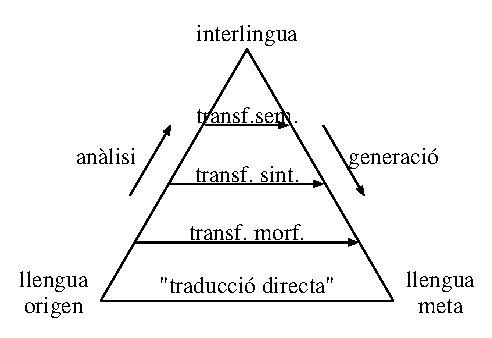
\includegraphics{triangle} \end{center} \caption{Cuanto más profundo y complejo es el análisis del texto origen, más sencilla es (menos esfuerzo requiere) la transferencia a la representación correspondiente de la lengua meta y más compleja la generación. El análisis del texto origen es tan profunda en los sistemas de interlingua clásicos que no es necesaria la transferencia.} \label{fg:triangle} \end{figure} 

Las interlinguas pueden ser de muchos tipos. Los sistemas clásicos usan representaciones estructurales más o menos complejas para representar las relaciones semánticas entre los elementos de la frase. 
% (de l'estil de les de la solució a l'exercici~\ref{exer:agradar}).  
Pero las interlinguas no tienen que ser necesariamente el resultado de un análisis profundo: lo que deben ser necesariamente es \emph{neutrales}; por ejemplo, algunos sistemas históricos como DLT \citep[cap.~17]{hutchins92b} usan como \emph{interlingua} una lengua \emph{pivote} ``natural'' como el esperanto, con anotaciones que resuelven algunas ambigüedades típicas.\footnote{Esta aproximación puede ser particularmente útil cuando las lenguas entre las que debe traducir el sistema tienen una gran similitud sintáctica y semántica, como en el caso de las lenguas románicas, con la excepción, quizás, del rumano.} 

En el intento de representar los significados de todas las frases de todas las lenguas, las interlinguas clásicas acabarían por ser "modelos del mundo''. Esto hace que, actualmente, sólo se hayan desarrollado sistemas de interlingua clásicos para ámbitos temáticos muy concretos. 

Una de las ventajas más importantes de todos los sistemas de interlingua respecto a los sistemas de transferencia es la facilidad con la que se puede añadir una lengua nueva a un sistema de traducción automática multilingüe. Imaginemos tres lenguas que denominaremos $L_1$, $L_2$ i $L_3$. Un sistema completo de transferencia que tradujera entre estas tres lenguas en los dos sentidos tendría tres módulos de análisis (que denominaremos $A_1$, $A_2$ y $A_3$), tres módulos de generación (que denominaremos $G_1$, $G_2$ y $G_3$) y seis módulos de transferencia (que denominaremos $T_{12}$, $T_{13}$, $T_{23}$, $T_{31}$, $T_{32}$ y $T_{21}$).\footnote{En general, para $N$ lenguas $L_1, L_2, \ldots, L_N$ habría $N$ modulos de análisis, $N$ modulos de generación y $N(N-1)$ modulos de transferencia.} Añadir un cuarto idioma $L_4$ al sistema comporta: \begin{itemize} \item Crear un nuevo módulo de análisis ($A_4$). \item Crear un nuevo modulo de generación ($G_4$). \item Construir 6 nuevos modulos de transferencia ($T_{14}$, $T_{24}$, $T_{34}$, $T_{41}$, $T_{42}$ y $T_{43}$). Nótese que para esta última fase son necesarios varios expertos bilingües en sistemas de transferencia.\footnote{En el caso general de añadir una lengua a un conjunto de $N$ lenguas, hacen falta $2N$ nuevos módulos de transferencia.} \end{itemize} La figura~\ref{fg:afetran} ilustra el coste de añadir $L_4$ al sistema de transferencia; \begin{figure} \begin{center} 

%TexCad Options
%\grade{\off}
%\emlines{\off}
%\beziermacro{\on}
%\reduce{\on}
%\snapping{\off}
%\quality{2.00}
%\graddiff{0.01}
%\snapasp{1}
%\zoom{1.00}
{\scriptsize \unitlength 0.80mm \linethickness{0.4pt} \begin{picture}(155.00,100.00) \put(110.00,10.00){\makebox(0,0)[cc]{$L_3$}} \put(110.00,25.00){\makebox(0,0)[cc]{$RA_3$}} \put(110.00,85.00){\makebox(0,0)[cc]{$RA_1$}} \put(110.00,100.00){\makebox(0,0)[cc]{$L_1$}} \put(80.00,55.00){\makebox(0,0)[cc]{$RA_2$}} \put(65.00,55.00){\makebox(0,0)[cc]{$L_2$}} \put(140.00,55.00){\makebox(0,0)[cc]{$RA_4$}} \put(155.00,55.00){\makebox(0,0)[cc]{$L_4$}} 

%\vector(152.00,57.00)(143.00,57.00)
\put(143.00,57.00){\vector(-1,0){0.2}} \put(152.00,57.00){\line(-1,0){9.00}} 

%\end
%\vector(143.00,53.00)(152.00,53.00)
\put(152.00,53.00){\vector(1,0){0.2}} \put(143.00,53.00){\line(1,0){9.00}} 

%\end
%\vector(108.00,97.00)(108.00,88.00)
\put(108.00,88.00){\vector(0,-1){0.2}} \put(108.00,97.00){\line(0,-1){9.00}} 

%\end
%\vector(112.00,88.00)(112.00,97.00)
\put(112.00,97.00){\vector(0,1){0.2}} \put(112.00,88.00){\line(0,1){9.00}} 

%\end
%\vector(68.00,53.00)(77.00,53.00)
\put(77.00,53.00){\vector(1,0){0.2}} \put(68.00,53.00){\line(1,0){9.00}} 

%\end
%\vector(77.00,57.00)(68.00,57.00)
\put(68.00,57.00){\vector(-1,0){0.2}} \put(77.00,57.00){\line(-1,0){9.00}} 

%\end
%\vector(108.00,22.00)(108.00,13.00)
\put(108.00,13.00){\vector(0,-1){0.2}} \put(108.00,22.00){\line(0,-1){9.00}} 

%\end
%\vector(112.00,13.00)(112.00,22.00)
\put(112.00,22.00){\vector(0,1){0.2}} \put(112.00,13.00){\line(0,1){9.00}} 

%\end
\put(104.00,93.00){\makebox(0,0)[cc]{$A_1$}} \put(116.00,93.00){\makebox(0,0)[cc]{$G_1$}} \put(72.00,61.00){\makebox(0,0)[cc]{$G_2$}} \put(72.00,49.00){\makebox(0,0)[cc]{$A_2$}} \put(148.00,49.00){\makebox(0,0)[cc]{$G_4$}} \put(148.00,61.00){\makebox(0,0)[cc]{$A_4$}} \put(116.00,17.00){\makebox(0,0)[cc]{$A_3$}} \put(104.00,17.00){\makebox(0,0)[cc]{$G_3$}} \put(108.00,82.00){\vector(0,-1){47.00}} \put(83.00,53.00){\vector(1,0){47.00}} \put(137.00,57.00){\vector(-1,0){47.00}} \put(112.00,28.00){\vector(0,1){47.00}} \put(137.00,57.00){\vector(-1,1){21.00}} \put(108.00,81.67){\vector(-1,-1){21.00}} \put(83.00,53.00){\vector(1,-1){21.00}} \put(112.00,28.00){\vector(1,1){21.00}} \put(83.00,53.00){\vector(1,1){21.00}} \put(112.00,28.00){\vector(-1,1){22.00}} \put(137.00,57.00){\vector(-1,-1){21.00}} \put(108.00,82.00){\vector(1,-1){22.00}} \put(130.00,70.00){\makebox(0,0)[cc]{$T_{41}$}} \put(125.00,35.00){\makebox(0,0)[cc]{$T_{34}$}} \put(90.00,40.00){\makebox(0,0)[cc]{$T_{23}$}} \put(95.00,75.00){\makebox(0,0)[cc]{$T_{12}$}} \put(100.00,65.00){\makebox(0,0)[cc]{$T_{21}$}} \put(120.33,45.33){\makebox(0,0)[cc]{$T_{43}$}} \put(120.00,65.00){\makebox(0,0)[cc]{$T_{14}$}} \put(100.00,45.00){\makebox(0,0)[cc]{$T_{32}$}} \put(100.00,50.00){\makebox(0,0)[cc]{$T_{24}$}} \put(120.00,60.00){\makebox(0,0)[cc]{$T_{42}$}} \put(116.00,45.33){\makebox(0,0)[cc]{$T_{31}$}} \put(105.00,65.00){\makebox(0,0)[cc]{$T_{13}$}} \put(45.00,10.00){\makebox(0,0)[cc]{$L_3$}} \put(45.00,25.00){\makebox(0,0)[cc]{$RA_3$}} \put(45.00,85.00){\makebox(0,0)[cc]{$RA_1$}} \put(45.00,100.00){\makebox(0,0)[cc]{$L_1$}} \put(15.00,55.00){\makebox(0,0)[cc]{$RA_2$}} \put(0.00,55.00){\makebox(0,0)[cc]{$L_2$}} 

%\vector(43.00,97.00)(43.00,88.00)
\put(43.00,88.00){\vector(0,-1){0.2}} \put(43.00,97.00){\line(0,-1){9.00}} 

%\end
%\vector(47.00,88.00)(47.00,97.00)
\put(47.00,97.00){\vector(0,1){0.2}} \put(47.00,88.00){\line(0,1){9.00}} 

%\end
%\vector(3.00,53.00)(12.00,53.00)
\put(12.00,53.00){\vector(1,0){0.2}} \put(3.00,53.00){\line(1,0){9.00}} 

%\end
%\vector(12.00,57.00)(3.00,57.00)
\put(3.00,57.00){\vector(-1,0){0.2}} \put(12.00,57.00){\line(-1,0){9.00}} 

%\end
%\vector(43.00,22.00)(43.00,13.00)
\put(43.00,13.00){\vector(0,-1){0.2}} \put(43.00,22.00){\line(0,-1){9.00}} 

%\end
%\vector(47.00,13.00)(47.00,22.00)
\put(47.00,22.00){\vector(0,1){0.2}} \put(47.00,13.00){\line(0,1){9.00}} 

%\end
\put(39.00,93.00){\makebox(0,0)[cc]{$A_1$}} \put(51.00,93.00){\makebox(0,0)[cc]{$G_1$}} \put(7.00,61.00){\makebox(0,0)[cc]{$G_2$}} \put(7.00,49.00){\makebox(0,0)[cc]{$A_2$}} \put(51.00,17.00){\makebox(0,0)[cc]{$A_3$}} \put(39.00,17.00){\makebox(0,0)[cc]{$G_3$}} \put(43.00,82.00){\vector(0,-1){47.00}} \put(47.00,28.00){\vector(0,1){47.00}} \put(43.00,81.67){\vector(-1,-1){21.00}} \put(18.00,53.00){\vector(1,-1){21.00}} \put(18.00,53.00){\vector(1,1){21.00}} \put(47.00,28.00){\vector(-1,1){22.00}} \put(25.00,40.00){\makebox(0,0)[cc]{$T_{23}$}} \put(30.00,75.00){\makebox(0,0)[cc]{$T_{12}$}} \put(35.00,65.00){\makebox(0,0)[cc]{$T_{21}$}} \put(35.00,45.00){\makebox(0,0)[cc]{$T_{32}$}} \put(51.00,45.33){\makebox(0,0)[cc]{$T_{31}$}} \put(40.00,65.00){\makebox(0,0)[cc]{$T_{13}$}} \end{picture} } \end{center} \caption{Coste de añadir una cuarta lengua $L_4$ a un sistema de transferencia. Las entidades $RA_1$ a $RA_4$ son las representaciones abstractas (tanto RALO como RALM) que usan los módulos de transferencia.} \label{fg:afetran} \end{figure} En cambio, en un sistema de interlingua no hay módulos de transferencia; un sistema trilingüe basado en una interlingua tendría sólo seis módulos: tres de análisis ($A'_1$, $A'_2$ y $A'_3$) y tres de generación ($G'_1$, $G'_2$ y $G'_3$). Queda claro que los módulos de análisis y de generación en estos sistemas son más complejos que en el caso de transferencia (puesto que tienen que hacer transformaciones hacia estructuras lingüísticamente neutrales), pero también está clara la ventaja del sistema de interlingua a la hora de añadir la lengua $L_4$: sólo hay que diseñar dos módulos nuevos, $A'_4$ y $G'_4$, y para diseñarlos sólo necesitamos una persona que conozca bien la lengua $L_4$ y la interlingua $I$ que usa el sistema. La figura~\ref{fg:afeinte} ilustra el coste de añadir $L_4$ al sistema. \begin{figure} \begin{center} 

%TexCad Options
%\grade{\off}
%\emlines{\off}
%\beziermacro{\on}
%\reduce{\on}
%\snapping{\off}
%\quality{2.00}
%\graddiff{0.01}
%\snapasp{1}
%\zoom{1.00}
\unitlength 1.00mm \linethickness{0.4pt} \begin{picture}(100.00,50.00) \put(60.00,30.00){\makebox(0,0)[cc]{$L_2$}} \put(80.00,10.00){\makebox(0,0)[cc]{$L_3$}} \put(80.00,50.00){\makebox(0,0)[cc]{$L_1$}} \put(100.00,30.00){\makebox(0,0)[cc]{$L_4$}} \put(80.00,30.00){\makebox(0,0)[cc]{$I$}} 

%\vector(78.00,33.00)(78.00,45.00)
\put(78.00,45.00){\vector(0,1){0.2}} \put(78.00,33.00){\line(0,1){12.00}} 

%\end
%\vector(82.00,47.00)(82.00,35.00)
\put(82.00,35.00){\vector(0,-1){0.2}} \put(82.00,47.00){\line(0,-1){12.00}} 

%\end
%\vector(83.00,32.00)(95.00,32.00)
\put(95.00,32.00){\vector(1,0){0.2}} \put(83.00,32.00){\line(1,0){12.00}} 

%\end
%\vector(97.00,28.00)(85.00,28.00)
\put(85.00,28.00){\vector(-1,0){0.2}} \put(97.00,28.00){\line(-1,0){12.00}} 

%\end
%\vector(82.00,27.00)(82.00,15.00)
\put(82.00,15.00){\vector(0,-1){0.2}} \put(82.00,27.00){\line(0,-1){12.00}} 

%\end
%\vector(78.00,13.00)(78.00,25.00)
\put(78.00,25.00){\vector(0,1){0.2}} \put(78.00,13.00){\line(0,1){12.00}} 

%\end
%\vector(77.00,28.00)(65.00,28.00)
\put(65.00,28.00){\vector(-1,0){0.2}} \put(77.00,28.00){\line(-1,0){12.00}} 

%\end
%\vector(63.00,32.00)(75.00,32.00)
\put(75.00,32.00){\vector(1,0){0.2}} \put(63.00,32.00){\line(1,0){12.00}} 

%\end
\put(70.00,36.00){\makebox(0,0)[cc]{$A'_2$}} \put(90.00,36.00){\makebox(0,0)[cc]{$G'_4$}} \put(90.00,24.00){\makebox(0,0)[cc]{$A'_4$}} \put(70.00,24.00){\makebox(0,0)[cc]{$G'_2$}} \put(74.00,40.00){\makebox(0,0)[cc]{$G'_1$}} \put(74.00,20.00){\makebox(0,0)[cc]{$A'_3$}} \put(86.00,20.00){\makebox(0,0)[cc]{$G'_3$}} \put(86.00,40.00){\makebox(0,0)[cc]{$A'_1$}} \put(10.00,30.00){\makebox(0,0)[cc]{$L_2$}} \put(30.00,10.00){\makebox(0,0)[cc]{$L_3$}} \put(30.00,50.00){\makebox(0,0)[cc]{$L_1$}} \put(30.00,30.00){\makebox(0,0)[cc]{$I$}} 

%\vector(28.00,33.00)(28.00,45.00)
\put(28.00,45.00){\vector(0,1){0.2}} \put(28.00,33.00){\line(0,1){12.00}} 

%\end
%\vector(32.00,47.00)(32.00,35.00)
\put(32.00,35.00){\vector(0,-1){0.2}} \put(32.00,47.00){\line(0,-1){12.00}} 

%\end
%\vector(32.00,27.00)(32.00,15.00)
\put(32.00,15.00){\vector(0,-1){0.2}} \put(32.00,27.00){\line(0,-1){12.00}} 

%\end
%\vector(28.00,13.00)(28.00,25.00)
\put(28.00,25.00){\vector(0,1){0.2}} \put(28.00,13.00){\line(0,1){12.00}} 

%\end
%\vector(27.00,28.00)(15.00,28.00)
\put(15.00,28.00){\vector(-1,0){0.2}} \put(27.00,28.00){\line(-1,0){12.00}} 

%\end
%\vector(13.00,32.00)(25.00,32.00)
\put(25.00,32.00){\vector(1,0){0.2}} \put(13.00,32.00){\line(1,0){12.00}} 

%\end
\put(20.00,36.00){\makebox(0,0)[cc]{$A'_2$}} \put(20.00,24.00){\makebox(0,0)[cc]{$G'_2$}} \put(24.00,40.00){\makebox(0,0)[cc]{$G'_1$}} \put(24.00,20.00){\makebox(0,0)[cc]{$A'_3$}} \put(36.00,20.00){\makebox(0,0)[cc]{$G'_3$}} \put(36.00,40.00){\makebox(0,0)[cc]{$A'_1$}} \end{picture} \end{center} \caption{Coste de añadir una cuarta lengua $L_4$ a un sistema de interlingua.} \label{fg:afeinte} \end{figure} 

\section{Sistemas de traducción automática basados en corpus} \label{ss:induc} Todas las técnicas de traducción automática descritas hasta ahora son de naturaleza \emph{deductiva}, es decir, están basadas en teorías y conocimientos lingüísticos sobre la traducción. Pero recientemente (sobre todo en los primeros años del tercer milenio) se está produciendo un crecimiento espectacular de las técnicas \emph{inductivas} de traducción automática, en las cuales el sistema \emph{aprende} automáticamente a traducir entre dos lenguas a partir de un corpus paralelo suficientemente grande de oraciones en LO acompañadas de su traducción a la LM (véase el apartado~\ref{ss:bitextos}). Estas aproximaciones inductivas también reciben el nombre de traducción \emph{automática basada en corpus}. 

\subsection{Sistemas de traducción automática estadística} \label{ss:tae} La principal técnica de traducción automática basada en corpus es la \emph{traducción automática estadística} (en inglés \emph{statistical machine translation}; SMT), que fue inventada hacia finales de los ochenta por un grupo de investigadores de IBM \citep{brown90j}; los sistemas actuales son una evolución de estos. 

A la hora de traducir hay una diferencia fundamental entre los sistemas basados en reglas o conocimiento y los sistemas estadísticos: mientras que los sistemas basados en reglas producen únicamente una traducción, los sistemas estadísticos generan una gran cantidad de \emph{hipótesis de traducción} (idealmente todas las posibles) y utilizan modelos estadísticos para \emph{puntuar} las hipótesis generadas y escoger la mejor de todas. Los principales modelos estadísticos que se usan para puntuar las hipótesis de traducción son el \emph{modelo de traducción} y el \emph{modelo de lengua}, los cuales se explican más abajo. La combinación de estos modelos hace que la hipótesis de traducción que recibe la puntuación \emph{global} más alta no sea necesariamente la hipótesis de traducción mejor según cada modelo por separado. 

\begin{figure} \centering

\begin{tabular}{p{6cm}|p{6cm}} \multicolumn{1}{c|}{\textbf{Inglés}} &\multicolumn{1}{c}{\textbf{Español}}\\ \hline

It has been exciting in many ways . &Ha sido un trabajo apasionante en varios sentidos . \\ \hline

As the shadow rapporteurs know , this has been my first report during my time in Parliament and it has been a good learning experience . &Como bien saben los ponentes alternativos , éste ha sido el primer informe en el que he trabajado durante mi mandato parlamentario , y me ha venido muy bien como experiencia formativa . \\ \hline

It has also been very challenging to work on three reports and therefore also with other rapporteurs . &También ha sido un gran desafío trabajar en tres informes , y por lo tanto con otros ponentes . \\ \hline

It has been exciting . &Ha sido emocionante . \\ \hline

\end{tabular} \caption{Oraciones paralelas inglés-español extraídas del corpus paralelo Europarl (\texttt{http://www.statmt.org/europarl/}) con las actas del Parlamento Europeo del período 1996--2011.} \label{fg:alinora} \end{figure} 

\begin{figure} \centering

\includegraphics[scale=0.5]{alin-paraules} \caption{Alineamiento entre las palabras de la oración en inglés \emph{The white bird decided to fly.} y las palabras de la oración en catalán \emph{El pardal blanc va decidir volar.}} \label{fg:alinpar} \end{figure} 

El \textbf{modelo de traducción} se aprende a partir de un corpus paralelo con las oraciones ya alineadas como el que se muestra en la figura \ref{fg:alinora}. Primeramente, se deben obtener los \emph{alineamientos entre las palabras} (véase un ejemplo en la figura \ref{fg:alinpar}) para después estimar el modelo de traducción a partir de estos alineamientos. 

\begin{figure}[tb] \centering \subfigure[\label{fg:pasosalin1}Inicialización: Todos los alineamientos son igualmente probables.]{\includegraphics[scale=0.5]{ibm1/ibm2}} 

%
\subfigure[\label{fg:pasosalin2}Primera iteración: El alineamiento entre \emph{yn} y \emph{gur} gana fuerza.]{\includegraphics[scale=0.5]{ibm1/ibm3}} 

\subfigure[\label{fg:pasosalin3}Segunda iteración: El alineamiento entre \emph{pifo} y \emph{ubhfo} gana fuerza.]{\includegraphics[scale=0.5]{ibm1/ibm4}} 

\subfigure[\label{fg:pasosalin4}Tercera y última iteración: La estructura de alineamiento que estaba ``oculta'' queda al descubierto.]{\includegraphics[scale=0.5]{ibm1/ibm5}} \caption{Ejemplo que ilustra el proceso iterativo que permite obtener el alineamiento entre las palabras de las oraciones de un corpus paralelo. En este ejemplo el corpus consta de tres oraciones paralelas en dos lenguas inventadas. Estas oraciones paralelas son: \emph{yn pifo}--\emph{gur ubhfo}, \emph{yn pifo oynapi}--\emph{gur juvga ubhfo} i \emph{yn sybe}--\emph{gur subjre}. El grosor de las líneas que conectan las palabras representa la probabilidad del alineamiento.} \label{fg:pasosalin} \end{figure} 

A pesar de que parece una tarea difícil para un ordenador, los alineamientos entre las palabras se pueden obtener automáticamente sin usar ningún conocimiento sobre las lenguas de los textos a alinear mediante un proceso iterativo. La figura \ref{fg:pasosalin} ilustra este proceso con un corpus pequeño de tres oraciones paralelas; si os fijáis, sin tener ningún conocimiento de las lenguas (porque han sido inventadas) las personas también somos capaces de obtener estos alineamientos. El proceso empieza asumiendo que, para cada oración paralela, todas las palabras de la oración en LM pueden ser traducción de cada una de las palabras de la oración en LO y, por lo tanto, les asigna la misma probabilidad. En cada iteración el programa alineador visita todas las oraciones paralelas del corpus y va refinando estas probabilidades hasta que la estructura de alineamiento queda definida. Este refinamiento se produce porque en cada iteración las probabilidades de la iteración anterior se usan para acumular evidencia en todo el corpus sobre la probabilidad de las correspondencias entre palabras y, además, porque las palabras que son traducción mutua suelen aparecer juntas en las mismas oraciones paralelas, lo cual no sucede si dos palabras no son traducción una de la otra. 

Una vez obtenidos los alineamientos entre las palabras, podemos aprender modelos probabilísticos que indican, por ejemplo, la probabilidad de que la traducción de una determinada palabra en una lengua sea la traducción de una determinada palabra en la otra (un modelo de traducción de palabras o diccionario bilingüe probabilístico), o la probabilidad de que la traducción de una secuencia (segmento) de palabras en una lengua sea la traducción de una secuencia (segmento) de palabras en la otra (un modelo de traducción de segmentos). Este último modelo lo usan los sistemas de traducción automática estadística basados en segmentos bilingües (en inglés \emph{phrase-based statistical machine translation}; \cite{koehnbook}), los cuales son los más usados en la actualidad. 

Pero para producir buenas traducciones no podemos usar el modelo de traducción únicamente porque las traducciones serían poco naturales, gramaticales y fluidas. El motivo es que el modelo de traducción no tiene en cuenta el orden en el que aparecen los segmentos traducidos en la LM, ni el contexto en el que aparecen los segmentos en LO a la hora de puntuar sus posibles traducciones. Estas deficiencias se mitigan parcialmente con el uso de un modelo de la LM. 

Un \textbf{modelo de lengua} es un modelo probabilístico que sirve para medir la verosimilitud de una oración o texto en LM; es decir, su fluidez o gramaticalidad.\footnote{Se asume que el modelo de lengua se aprende de textos naturales y gramaticalmente correctos en LM.} Estos modelos se aprenden de forma automática a partir de un corpus de texto en LM y se basan en contar la frecuencia de segmentos de longitud fija, normalmente segmentos de hasta cinco palabras, para evitar asignar una verosimilitud nula a oraciones que, a pesar de que son correctas, no aparecen en los corpus de entrenamiento.\footnote{Para evitar asignar verosimilitudes nulas a una oración, además de utilizar segmentos de pocas palabras, estos modelos también usan técnicas de suavizado (en inglés \emph{smoothing}) de las probabilidades.} El modelo de lengua tiene en cuenta el orden de las palabras y, por lo tanto, asigna una verosimilitud mayor a la oración \emph{M'agrada menjar pernil del bo} que a la oración \emph{del bo menjar pernil M'agrada}, a pesar de que contienen los mismos segmentos de texto (\emph{del bo}, \emph{menjar pernil} y \emph{M'agrada}). Además, tiene en cuenta, a pesar de que indirectamente, el contexto en el que aparecen las palabras en LM, de forma que asigna una verosimilitud mayor a la oración en español (LM) \emph{No piensa con la cabeza} que a la oración \emph{No piensa con el cabo}, donde los segmentos \emph{la cabeza} y \emph{el cabo} son dos posibles traducciones del segmento en catalán \emph{el cap} que aparece en la oración en LO \emph{No pensa amb el cap}. 

\begin{persabermes}{sistemas de traducción automática estadística} Además de los modelos de traducción y de la LM, los sistemas de traducción automática estadística basados en segmentos bilingües combinan otros modelos para establecer la puntuación global de una hipótesis de traducción. A continuación se describen muy brevemente estos modelos y para qué se usan: \begin{description} \item[Modelo de reordenamiento léxico:] Su función es modelar diferentes operaciones de reordenamiento que se pueden hacer a la hora de disponer las traducciones de los segmentos en LO. Las probabilidades de estas operaciones dependen de los segmentos concretos que se están reordenando y son tres: traducción monótona (cuando no hay reordenamiento), reordenamiento (cuando la posición de la traducción del segmento en cuestión y la del anterior se intercambian) y traducción discontinua (cuando la traducción del segmento se mueve a otra posición en la oración en LM; es decir, cuando no es ninguna de las otras dos operaciones). \item[Ponderación léxica:] Los segmentos usados para traducir pueden ser muy largos (normalmente hasta 7 palabras), lo que hace muy difícil estimar bien su probabilidad de traducción porque los segmentos largos suelen aparecer pocas veces en los corpus de entrenamiento; esto hace necesario el uso de otro modelo para estimar la calidad de los segmentos bilingües. Este modelo usa las probabilidades de traducción entre las palabras (un diccionario bilingüe probabilístico) para obtener un indicador de la calidad de los segmentos bilingües. Por ejemplo, la calidad del segmento bilingüe (\emph{la comissió de balanços de finançament}, \emph{the funding balance comission}), donde el alineamiento entre las palabras es \emph{la}--\emph{the}, \emph{comissió}--\emph{comission}, \emph{balanços}--\emph{balance} y \emph{finançament}--\emph{funding}, depende de las probabilidades de traducción de las palabras que han sido alineadas. \item[Número total de palabras de la oración:] Cuando se puntúan las hipótesis de traducción se multiplican muchas probabilidades, es decir valores entre 0 y 1, de forma que cuanto más larga sea una traducción más probabilidades se multiplican y más fácil es llegar a tener una puntuación muy cerca de cero. Esto hace que los sistemas prefieran las traducciones cortas. Para evitar esto se introduce un modelo que cuenta el número de palabras en la hipótesis de traducción y que hace que tenga relación con el número de palabras de la oración origen. \item[Número de segmentos:] Este modelo es similar al anterior, pero contando el número de segmentos bilingües que se han usado para producir una hipótesis de traducción. Cuanto más largos sean los segmentos, menos segmentos se usarán y más contexto tendrán; y al revés, cuanto más cortos sean los segmentos más segmentos harán falta para producir la hipótesis de traducción. \end{description} 

Todos estos modelos (y los anteriores) se combinan para obtener una puntuación global para cada hipótesis de traducción y poder escoger así la mejor. Esta combinación se hace asignando un peso (importancia) a cada modelo que se obtiene mediante un proceso automático (\emph{tuning}) que intenta maximizar la \emph{calidad} de las traducciones proporcionadas por el sistema al traducir un corpus de \emph{desarrollo}. 

Consultad el libro de \citet{koehnbook} para saber más sobre los modelos que se usan para traducir, el proceso de \emph{tuning} y las medidas automáticas de la calidad que usan. \end{persabermes} 

\begin{persabermes}{sistemas basados en corpus} Ha habido otras aproximaciones inductivas a la traducción automática, como, por ejemplo, los sistemas de \emph{traducción automática basada en ejemplos}, a pesar de que a estas alturas ya no se usan. La \emph{traducción automática basada en ejemplos} intenta construir \emph{plantillas} de traducción a partir de los ejemplos observados en el corpus de oraciones paralelas y \emph{generalizarlas} para que sirvan en nuevas situaciones. Por ejemplo, si sabemos que el sustantivo inglés \emph{ski} se traduce por \emph{esquí} y que la locución sustantiva \emph{ski station} se traduce por \emph{estació d'esquí} podemos generalizar esta última locución sustituyendo \emph{ski} por cualquier otros sustantivo $N$, de forma que la traducción de ``$N$ \emph{station}'' es ``estació de $N$''; así, si la traducción de \emph{train} es \emph{tren}, la traducción de \emph{train station} es \emph{estació de tren}, etc. (ejemplo extraído de \citealt{carl01j}). Fijaos que la traducción automática basada en ejemplos puede necesitar que la muestra de frases y traducciones esté, además, anotada lingüísticamente (en el ejemplo, indicando qué palabras o estructuras funcionan como un nombre). \end{persabermes} 

\section{Cuestiones y ejercicios} Los ejercicios marcados con (*) son más difíciles. 

\begin{enumerate} \item Los sistemas de traducción palabra por palabra pueden cometer, por ejemplo, errores en la concordancia de género o de número. Elegid dos lenguas $L_1$ y $L_2$ y poned al menos dos ejemplos de traducciones palabra por palabra de $L_1$ a $L_2$ con problemas de concordancia. 

\item (*) \label{ex:cascat} CasCat es un sistema de traducción automática del español al catalán que usa reglas que reordenan secuencias de formas léxicas según las categorías léxicas. Las reglas se aplican de la manera usual: de izquierda a derecha, reordenando la secuencia más larga posible, y sin que se solapen las áreas reordenadas. He aquí algunas frases españolas con {\em cuyo}, las traducciones producidas por CasCat, y, donde la traducción es incorrecta, una alternativa aceptable. \begin{enumerate} \item \emph{La chica cuyos compañeros murieron es china} \newline{\em La noia els companys de la qual van morir és xinesa} \item \emph{La chica cuyos compañeros de clase murieron es china} \newline \emph{La noia els companys de classe de la qual van morir és xinesa} \item \emph{La chica cuyos compañeros mayores murieron es china} \newline \emph{La noia els companys grans de la qual van morir és xinesa} \item \emph{La chica cuyos compañeros de clase de francés murieron es china} \newline \emph{*La noia els companys de classe de la qual de francès van morir és xinesa} \newline (\emph{La noia els companys de classe de francès de la qual van morir és xinesa}) \item \emph{La chica cuyos compañeros mayores de classe murieron es china} \newline \emph{*La noia els companys grans de la qual de classe van morir és xinesa} \newline (\emph{La noia els companys grans de classe de la qual van morir és xinesa}) \item \emph{La chica cuyos compañeros mayores de clase de francés murieron es china} \newline \emph{*La noia els companys grans de la qual de classe de francès van morir és xinesa} \newline(\emph{La noia els companys grans de classe de francès de la qual van morir és xinesa}) \end{enumerate} Las traducciones inaceptables están marcadas con un asterisco. Proponed un conjnto de reglas de reordenamiento que explican el conjunto de traducciones observado. ¿En qué casos se '' rompen" sintagmas? 

\item La multinacional WorldTrans ha decidido ampliar su sistema de traducción automática multilingüe LetTrans (que traduce correspondencia comercial entre cualesquier dos lenguas de un grupo de quince) y añadir la capacidad de traducir del suajili a las quince lenguas y de las quince lenguas hacia el suahili. En una oferta de trabajo, WorldTrans pide expertos en suajili, pero no pide ningún experto en traducción entre suahili y ninguna de las quince lenguas. ¿Qué clase de sistema de traducción automática es LetTrans? Justificad vuestra respuesta. 

\item (*) Imaginad que tenéis un sistema de traducción automática que trabaja con dos lenguas, digamos $A$ y $B$, en los dos sentidos de traducción: $A{\rightarrow}B$ y $B{\rightarrow}A$, que traducimos un texto origen $T$ en lengua $A$ a la lengua $B$ mediante este traductor automático, generando un texto $T'$, y que después usamos este mismo sistema para traducir $T'$ de nuevo a la lengua $A$; denominaremos $T''$ el nuevo texto en lengua $A$. \begin{equation} T \stackrel{\scriptsize A\rightarrow B}{\longrightarrow}T'\stackrel{\scriptsize B\rightarrow A}{\longrightarrow} T'' \end{equation} El texto $T''$ será previsiblemente diferente del texto $T$. Elegid dos lenguas $A$ y $B$ e indicad qué cambios son previsibles, clasificándolos según la naturaleza lingüística de los fenomens que han causado los cambios, explicando la razón del resultado si hace falta con un ejemplo. Tenéis que indicar \emph{tres tipos diferentes} de cambio. 

\item (*) Imaginad que sois parte de un equipo de desarrollo de un sistema de traducción automática del inglés al catalán basado en la estrategia de transferencia morfológica avanzada (apartado~\ref{s3:STMorf}). Los informáticos del proyecto os piden consejo sobre las reglas de reordenamiento del sistema, puesto que, por motivos técnicos, sólo pueden añadir tres. 

Indicad cuáles serían las 3 reglas que propondríais, teniendo en cuenta que tienen que producir, como mínimo, tres oraciones bien traducidas en el corpus de oraciones siguientes (la traducción ideal se indica entre paréntesis, a pesar de que no siempre se podrá conseguir): \begin{enumerate} \item \emph{A dark autumn night} (\emph{Una nit fosca de tardor}) \item \emph{A high tide} (\emph{Una marea alta}) \item \emph{A magic dark silhouette} (\emph{Una silueta fosca màgica}) \item \emph{An autumn tide} (\emph{Una marea de tardor}) \item \emph{A dark magic silhouette} (\emph{Una silueta màgica fosca}) \item \emph{A dark autumn high tide} (\emph{Una marea alta de tardor fosca}) \item \emph{A dark night} (\emph{Una nit fosca}) \end{enumerate} 

Dejad a un lado la concordancia y centraos sólo en los reordenamientos. Señalad cuál sería la traducción del sistema para todas las oraciones anteriores usando el conjunto de reglas que habéis propuesto. 

\item ¿Cuál es la operación inversa del análisis morfológico? \begin{enumerate} \item La obtención de la forma léxica de una palabra a partir de la forma superficial. \item La generación morfológica. \item La transferencia morfológica. \end{enumerate} 

\item La traducción automática por transferencia es siempre... \begin{enumerate} \item ... morfológica. \item ... directa. \item ... indirecta. \end{enumerate} 

\item (*) Dos traducciones posibles de la palabra catalana \emph{cap} al espanyol son \emph{cabe} o \emph{cabeza}. ¿Cómo podria hacer la elección adecuada un sistema de traducción automática? \begin{enumerate} \item Poniendo la traducción más probable, basada en las frecuencias de uso de las palabras. \item Usando información morfosintáctica, puesto que en la posición concreta de la frase podría ir sólo un verbo o un sustantivo. \item No podría, porque las dos traducciones son siempre posibles en cualquier frase. \end{enumerate} 

\item ¿Cuáles de las siguientes representaciones intermedias son más costosas de obtener a partir de las frases? \begin{enumerate} \item Los árboles de análisis sintáctico correspondientes. \item Las secuencias de categoróas morfológicas correspondientes. \item Las estructuras semánticas superficiales corresponendientes.re \end{enumerate} 

%\item Només una d'aquestes operacions és esperable en una situació
%  normal de traducció automàtica. Quina?
%  \begin{enumerate}
%  \item La postedició en un sistema de traducció automàtica usat per a
%    l'assimilació.
%  \item Una fase complexa de transferència en un sistema
%    d'interlingua.
%  \item La preedició en un sistema de traducció automàtica usat per a
%    la disseminació.
%  \end{enumerate}
\item El análisis morfológico toma una oración y... \begin{enumerate} \item ... produce un árbol de análisis. \item ... produce, para cada palabra, todas las formas superficiales correspondientes. \item ... produce, para cada palabra, todas las tripletas lema--categoría--información morfológica posibles. \end{enumerate} 

\item ¿Cuáles son las fases básicas de un sistema de traducción automática indirecta? \begin{enumerate} \item Análisis, generación y traducción. \item Análisis, transferencia y generación. \item Análisis y transferencia. \end{enumerate} 

\item ¿Cuáles de los siguientes tipos de traducción automática facilitan más la adición de una nueva lengua? \begin{enumerate} \item Los sistemas de transferencia morfológica avanzada. \item Los sistemas de transferencia semántica superficial. \item Los sistemas de\emph{interlingua}. \end{enumerate} 

\item ¿Cuál de los siguientes tipos sistema de traducción automática tienen la fase de transferencia más sencilla posible? \begin{enumerate} \item Los sistemas de transferencia morfológica avanzada. \item Los sistemas de transferencia semántica superficial. \item Los sistemas de\emph{interlingua}. \end{enumerate} 

\item Primeramente, elegid un idioma meta (francés, inglés o alemán) y un idioma origen (catalàn o español). Después, para los idiomas elegidos, dad un ejemplo de traducción palabra a palabra inaceptable en \emph{tres} de estos cinco casos: \begin{enumerate} \item homografía mal resuelta de una palabra \item polisemia mal resuelta de una palabra \item problemas de concordancia \item ambigüedad estructural mal resuelta \item problemas con el orden de las palabras \end{enumerate} 

\item \emph{Interlingua}, además de ser el nombre de la representación intermedia de los sistemas indirectos sin transferencia, es el de una lengua artificial básicamente de raíz latina, con una flexión simplificada, y con un vocabulario diseñado para ser comprensible a muchos europeos. Una característica importante de interlingua es que los determinantes (\emph{un}, \emph{le}, \emph{alcun}, \emph{iste}, \emph{mi}, \emph{tu}, etc.) y los adjetivos son invariables. Los plurales de los nombres se hacen con  \emph{-s} o \emph{-es}. Imaginad que tenemos un sistema de transferencia morfológica avanzada que traduce de interlingua al catalán (o al español) usando estas cuatro reglas: \begin{itemize} \item[$R_1$] detecta \textbf{det}--\textbf{n} y escribe \textsf{trad}(\textbf{det})--\textsf{trad}(\textbf{n}), haciendo concordar \textsf{trad}(\textbf{det}) en género y en número con \textsf{trad}(\textbf{n}) \item[$R_2$] detecta \textbf{det}--\textbf{n}--\textbf{adj} y escribe \textsf{trad}(\textbf{det})--\textsf{trad}(\textbf{n})-\textsf{trad}(\textbf{adj}), haciendo concordar \textsf{trad}(\textbf{det}) y \textsf{trad}(\textbf{adj})en género y en número con \textsf{trad}(\textbf{n}) \item[$R_3$] detecta \textbf{n}--\textbf{adj} y escribe \textsf{trad}(\textbf{n})--\textsf{trad}(\textbf{adj}), haciendo concordar \textsf{trad}(\textbf{adj}) en género y en número con \textsf{trad}(\textbf{n}) \item[$R_4$] detecta \textbf{adj}--\textbf{n} y escribe \textsf{trad}(\textbf{n})--\textsf{trad}(\textbf{adj}), haciendo concordar \textsf{trad}(\textbf{adj}) en género y en número con \textsf{trad}(\textbf{n}) \end{itemize} Si no se puede usar información de concordancia, la traducción de los determinantes y los adjetivos se hace en masculino singular. Indica qué traducciones al catalán (o al español) producirá este sistema para las frases siguientes y por qué: \begin{enumerate} \item \emph{Un longe viage} \item \emph{Un longe viages} \item \emph{Un viages longe} \item \emph{Longe viages} \item \emph{Un governamento non democratic} \item \emph{Un governamentos non democratic} \item \emph{Tu melior ideales} \item \emph{Un bon solution} \end{enumerate} 

\item (*) La traducción de una oración se puede ver como una interpretación de esta (es decir, como la expresión en la lengua meta de su significado). El \emph{principio de composicionalidad semántica} postula que la interpretación de una oración se construye combinando las interpretaciones de las palabras siguiendo precisamente las agrupaciones sucesivas (constituyentes) que indica el árbol de análisis sintáctico de la oración, partiendo de las palabras y yendo hacia la raíz del árbol. Indicad en qué tipo (o tipos) de sistema de traducción automática encontramos un diseño que aplica, exactamente o aproximadamente, el principio de composicionalidad. Razonad brevemente la respuesta. 

\item \label{ex:zkanagg} El software que llevan instalado las naves de la confederación galáctica incluye un programa que traduce una de las lenguas mayoritárias del planta Zkanagg, el tazkannwat, al catalán. El sistema es un sistema de transferencia morfológica avanczada estándar, que lee los textos de izquierda a derecha, palabra a palabra, busca en la entrada los patrones de categorías léxicas que contiene en su catálogo, selecciona el más largo, reordena y concuerda las palabras del patrón, los escribe, y continúa después de la zona reordenada. Algunas traducciones son erroneas porque el sistema no tiene un catálago demasiado completo de reglas.	  Fijaos en los ejemplos y decid cuáles son los patrones que detecta y cuáles las reglas de reordenamiento asociadas.
   \begin{example} 
   \gll Thlong u knaar uw phlagyw. 
        {Adquirió} el navegante el-OBJ control-OBJ 
   \glt TA: El navegante adquirió el control (correcta). 
   \glend
   \end{example} 
   \begin{example} 
   \gll Thlong u knaar qimratt uw phlagyw. 
        {Adquirió} el navegante estelar el-OBJ control-OBJ 
   \glt TA: El navegante estelar adquirió el control (correcta). 
   \glend
   \end{example} 
   \begin{example} 
   \gll Thlong u knaar na Zkannag uw phlagyw. 
        {Adquirió} el navegante de Zkannag el-OBJ control-OBJ 
   \glt TA: El navegante de Zkannag adquirió el control (correcta). 
   \glend
   \end{example} 
   \begin{example} 
   \gll Thlong u knaar qimratt na Zkannag uw phlagyw. 
        {Adquirió} el navegante estelar de Zkannag el-OBJ control-OBJ 
   \glt TA: *El navegante estelar adquirió de Zkannag el control. 
   \glt Correcta: El navegante estelar de Zkannag adquirió el control.
   \glend
   \end{example} 

% \item \label{exer:agradar} Les estructures sintàctiques usades per diverses llengües a
%   l'hora d'expressar el fet que alguna acció agrada a algú són molt
%   diverses. La frase ``m'agrada nadar'' té una estructura sintàctica molt
%   diferent en anglés (\ref{ex:angles}) i en alemany (\ref{ex:alemany}).
% \begin{example}
% \gll Peter likes swimming.
%      Peter s'estima nadant.
% \glt\glend
% \label{ex:angles}
% \end{example}
% \begin{example}
% \gll Peter schwimmt gern.
%      Peter nada {amb gust}.
% \glt\glend
% \label{ex:alemany}
% \end{example}
% Altre exemple el tenim en la frase  ``li diuen Joan'':
% \begin{example}
% \gll He is called Joan.
%      Ell és anomenat Joan.
% \glt\glend
% \label{ex:angles2}
% \end{example}
% \begin{example}
% \gll Er hei{\ss}t Joan.
%      Ell {s'anomena}  Joan.
% \glt\glend
% \label{ex:alemany2}
% \end{example}
% En canvi, les estructures que serveixen per a expressar altres
% conceptes poden ser completament paral·leles. Quines conseqüències té
% això per al disseny d'un sistema de traducció automàtica de
% transferència sintàctica entre llengües amb aquestes característiques?
% Com es podrien evitar els problemes observats?
\item Las palabras no son todas igualmente frecuentes en los textos. De hecho, si ordenamos las palabras de un gran corpus de texto real (de cualquier tipo y de cualquier idioma) por el número de veces que aparecen, empezando por la más frecuente, el número de apariciones se reduce dramáticamente según vayamos bajando por la lista. Típicamente, la palabra más frecuente puede llegar a constituir el 10\% de todo el texto, pero el segundo sólo cubre alrededor del 5\%, el tercero alrededor del 3\%, etc.; cuando llegamos a la 100.ª palabra más frecuente ya tenemos que hablar del 0,1\% (una vez cada 1.000 palabras), y si llegamos a la posición 1000, del 0,01\% (una vez cada 10.000 palabras). En resumen, la distribución no es nada homogénea: unas pocas palabras son las más frecuentes y la mayoría son muchísimo menos frecuentes. De hecho, es típico que la mayoría de las palabras sean \emph{hapax legomena}, es decir, palabras que han aparecido sólo una vez en todo el corpus. ¿Si hubiérais de supervisar la contrucción de los diccionarios de un sistema de traducción automática, para qué os pordrían servir estas constataciones estadísticas? 

\item (*) \label{ex:postres} Los sistemas de traducción automática entre dos lenguas con sintaxis similar no necesitan hacer demasiados reordenamientos porque el orden de las palabras no varía demasiado de una lengua a otra. A pesar de esto, la traducción palabra por palabra no es practicable porque el género y el número gramatical de algunos sustantivos varía y los adjetivos, artículos, etc. que lo acompañan no concordarían correctamente: cast. {\em una señal muy clara\/} $\rightarrow$ cat. *{\em una senyal molt clara} (correcto: {\em un senyal molt clar\/}); cast. {\em me gusta la leche fría} $\rightarrow$ ital. *{\em mi piace la latte fredda\/} (correcto: {\em mi piace il latte freddo}). Una manera de identificar zonas donde se tiene que establecer la concordancia es detectar secuencias de palabras, de manera similar a cómo se hace en los sistemas de transferencia morfológica, pero sin reordenarlas. Por ejemplo, detectar la secuencia {\bf art}--{\bf subst} puede servir para propagar el género y el número del sustantivo al artículo. Fijaos en las frases españolas siguientes y las traducciones al catalán hechas por un sistema que usa esta estrategia y deducid cuáles son las secuencias que detecta y cuales no. Justificad vuestra respuesta. \begin{enumerate} \item \emph{Nos ofreció un postre} $\rightarrow$ \emph{Ens va oferir unes postres\/} \item \emph{Nos ofreció un postre buenísimo} $\rightarrow$ \emph{Ens va oferir unes postres boníssimes\/} \item \emph{Nos ofreció un buen postre} $\rightarrow$ \emph{*Ens va oferir un bon postres\/} \item \emph{Nos ofreció un postre típico buenísimo\/} $\rightarrow$ \emph{*Ens va oferir unes postres típiques boníssim\/} \item \emph{Nos ofreció un postre muy bueno} $\rightarrow$ \emph{*Ens va oferir unes postres molt bo\/} \end{enumerate} 

\item Indica cuál de estas afirmaciones es falsa. \begin{enumerate} \item Los sistemas de transferencia sintáctica hacen análisis sintáctico sin hacer análisis morfológico. \item Los sistemas de transferencia sintáctica sólo usan información bilingüe en una de las tres fases. \item La fase de transferencia de un sistema de transferencia sintáctica realiza transformaciones de árboles de análisis sintáctico de acuerdo con reglas determinadas. \end{enumerate} 

\item Elige la secuencia que está en el orden temporal correcto: \begin{enumerate} \item Preedición, postedición, traducción por transferencia, diseminación. \item Preedición, traducción por transferencia, diseminación, postedición. \item Preedición, traducción por transferencia, postedición, diseminación. \end{enumerate} 

\item ¿En qué tipo de sistema de traducción automática tendrían básicamente la misma representación las frases \emph{David és vist per Lluc} y \emph{Lluc veu David}? \begin{enumerate} \item En un sistema de transferencia morfológica. \item En un sistema de transferencia semántica o de interlingua clásico. \item En un sistema de transferencia sintáctica. \end{enumerate} 

\item ¿Cuántas lenguas naturales tiene que conocer el equipo de expertos que tiene que incorporar una nueva lengua a un sistema de traducción automática basado en interlingua que ya tiene 7? \begin{enumerate} \item Siete. \item Una. \item Ocho. \end{enumerate} 

\item Cuanto más profundo es el análisis en un sistema de traducción automática{\ldots} \begin{enumerate} \item {\ldots}más compleja es la transferencia. \item {\ldots}más sencilla es la generación. \item {\ldots}más sencilla es la transferencia. \end{enumerate} 

\item Si una oración tiene sólo una ambigüedad léxica pura, tiene sólo un único árbol de análisis sintáctico. Por lo tanto, si se traduce esta oración con un sistema de traducción automática indirecta por transferencia sintáctica{\ldots} \begin{enumerate} \item {\ldots}el sistema se bloqueará porque sólo opera a nivel sintáctico \item {\ldots}la ambigüedad léxica no afecta al resultado porque no afecta a la sintaxis \item {\ldots}puede todavía producirse un error en la traducción a causa de la ambigüedad léxica de transferencia \end{enumerate} 

% \item Indiqueu quina d'aquestes afirmacions és certa.
%   \begin{enumerate}
%   \item Els sistemes de transferència semàntica fan anàlisi semàntica
%     sense fer anàlisi sintàctica.
%   \item Els sistemes de transferència sintàctica usen únicament
%     informació monolingüe en dues de les tres fases.
%   \item La fase de transferència d'un sistema de transferència
%     sintàctica es realitza basant-se en el fet que els arbres
%     d'anàlisi sintàctica són invariables.
%   \end{enumerate}
\item Un sistema de traducción automática por transferencia traduce en cualquier sentido entre cuatro lenguas. Si queremos añadir una quinta lengua porque traduzca en cualquier sentido entre cinco lenguas, ¿cuántos módulos nuevos hay que escribir? \begin{enumerate} \item 4 de transferencia, uno de análisis y uno de generación \item 5 de transferencia, uno de análisis y uno de generación \item 8 de transferencia, uno de análisis y uno de generación \end{enumerate} 

\item ¿En cuál de las tres fases de un sistema de transferencia se usan los diccionarios bilingües? \begin{enumerate} \item En la de análisis. \item En la de generación \item En la de transferencia. \end{enumerate} 

\item Un amigo mío ha diseñado un sistema de traducción automática entre el español y el portugués, pero a pesar de que me asegura que no ha programado ningún tratamiento de la ambigüedad estructural, su sistema traduce perfectamente un montón de oraciones con este tipo de ambigüedad. ¿Esto es posible? \begin{enumerate} \item No. Probablemente ha diseñado también un módulo de preedición y el sistema elimina automáticamente cualquier causa de ambigüedad. \item Sí, esto puede ocurrir cuando se dan los llamados \emph{pases gratuitos}; seguro que, si insistimos, encontraremos alguna oración mal traducida. \item Sí, si se trata de oraciones en las que esta ambigüedad se debe a palabras polisémicas y el programa tiene un diccionario bastante completo. \end{enumerate} 

\item Los informáticos que participan en el diseño de un sistema de traducción por interlingua te informan de que cada una de las fases del sistema se tiene que ejecutar en un ordenador diferente. ¿Cuántos ordenadores tenemos que comprar? \begin{enumerate} \item Dos, uno para la fase de análisis y otro para la de generación. \item Dos, uno para la fase de análisis y otro para la de transferencia. \item Tres, uno para la fase de análisis, otro para la de transferencia y un tercero para la de generación. \end{enumerate} 

\item ¿Cuántos módulos de análisis y de generación tenemos que añadir en total a un sistema basado en transferencia que ahora mismo permite traducir entre 4 lenguas, si queremos incorporar una lengua más de forma que el sistema pueda traducir (tanto en un sentido como en el otro) entre todas las lenguas existentes y la nueva? \begin{enumerate} \item 2 \item 4 \item 6 \end{enumerate} 

\item Si una forma superficial tiene sólo una forma léxica, pero dos posibles traducciones a otra lengua{\ldots} \begin{enumerate} \item {\ldots} se trata de una palabra homófona. \item {\ldots} se trata de una palabra homógrafa. \item {\ldots} probablemente un sistema automático tendrá que recurrir a información estadística o reglas sobre el contexto para elegir una de las soluciones. \end{enumerate} 

\item (*) En un corpus de textos en español sobre economía de 925.461 palabras estudiamos cuándo aparecen palabras conjuntamente. En concreto, y para poner un ejemplo, estudiamos pares de palabras gramaticalmente válidas donde la primera palabra aparece unas 400 veces en total en el corpus y la segunda palabra  aparece unas 200. Fijaos en la tabla \ref{tb:corpus} de frecuencias de aparición de algunos pares. A pesar de que tanto la primera palabra como la segunda palabra de cada par tienen frecuencias similares, en algún caso las frecuencias de aparición conjunta son muy elevadas y en otros casos son mucho más reducidas. ¿Podríais explicar la causa de esta variación? ¿Para qué aplicación de la informática a la traducción podrían servir los resultados de un estudio numérico como este? \begin{table*} \begin{center} \begin{tabular}{lr|lr|lr} \hline\hline \multicolumn{2}{c|}{\textsf{Primera palabra}} &\multicolumn{2}{c|}{\textsf{Segunda palabra}} &\multicolumn{2}{c}{\textsf{Expresión}} \\ \hline

\emph{fondos} &(410) &\emph{estructurales} &(203) &\emph{fondos estructurales} &(63) \\ \emph{precio} &(415) &\emph{máximo} &(202) &\emph{precio máximo} &(2) \\ \emph{algunos} &(403) &\emph{sectores} &(211) &\emph{algunos sectores} &(1) \\ \emph{hacia} &(409) &\emph{ellos} &(204) &\emph{hacia ellos} &(0) \\ \emph{otra} &(411) &\emph{crisis} &(203) &\emph{otra crisis} &(0) \\ \hline

\end{tabular} \end{center} \caption{Frecuencias de aparición de pares de palabras sobre economía.} \label{tb:corpus} \end{table*} 

\item Elige una lengua origen (catalán, español, inglés, francés o alemán) y una lengua meta (catalán, español, inglés, francés o alemán) y da \emph{tres} ejemplos de frases que se pueden traducir aceptablemente \emph{palabra por palabra} pero tales que si cambiamos \emph{una palabra} de las frases por otro de la misma categoría, la traducción \emph{palabra por palabra} resulta incorrecta. En cada una de las frases, la razón lingüística por la cual la segunda traducción es incorrecta tiene que ser diferente. 

\item (*) Estudiad los siguientes sintagmas nominales en maorí (una lengua polinesia hablada en Nueva Zelanda): 

     \begin{example} 
     \gll Te whare. 
          \textsf{Art.\ def.\ sg.} casa . 
     \glt La casa. 
     \glend
     \end{example} 

     \begin{example} 
     \gll Ng\={a} whare . 
          \textsf{Art.\ def.\ pl.} casa . 
     \glt Las casas. 
     \glend
     \end{example} 

     \begin{example} 
     \gll Te whare nui . 
          \textsf{Art.\ def.\ sg.} casa grande. 
     \glt La casa grande. 
     \glend
     \end{example} 

     \begin{example} 
     \gll Te whare nui o te aroha . 
          \textsf{Art.\ def.\ sg.} casa grande de \textsf{Art.\ def.\ 
          sg.} amor . 
     \glt La casa grande del amor. 
     \glend
     \end{example} 

     \begin{example} 
     \gll Ng\={a} whare nui . 
          \textsf{Art.\ def.\ pl.} casa grande. 
     \glt Las casas grandes. 
     \glend
     \end{example} 

Como en los ejemplos, en maorí la mayoría de los nombres y adjetivos son invariables. Imaginad que sois parte de un equipo de desarrollo de un sistema de traducción automática del maorí al catalán (o al español) basado en la estrategia que hemos denominado en el apartado~\ref{s3:STMorf} \emph{transferencia morfológica avanzada}.\footnote{Es decir, lee las oraciones palabra por palabra de izquierda a derecha y hace el análisis morfológico de cada palabra, prueba a detectar la secuencia más larga de palabras que concuerda con alguna secuencia de categorías léxicas que tiene en su catálogo, procesa la secuencia, y continúa inmediatamente después de la secuencia procesada.} Especifica completamente \emph{dos} reglas (indicando posibles reordenamientos y operaciones para asegurar la concordancia) que permiten dar la traducción correcta de las oraciones de arriba y de las siguientes. No os preocupéis de la contracción preposición--artículo. 

\begin{example} \emph{Ng\={a} whare nui o te aroha} (Las casas grandes del amor) \end{example} \begin{example} \emph{Te hau o te aroha} (El viento del amor) \end{example} \begin{example} \emph{Ng\={a}pukapuka o te whare} (El libro de la casa) \end{example} \begin{example} \emph{Ng\={a} ingoa o te pukapuka nui} (Los nombres del libro grande) \end{example} \begin{example} \emph{Te ingoa o ng\={a} whare} (El nombre de las casas) \end{example} 

\item Se quiere construir un sistema de traducción automática que traduzca entre cualquiera de las dos lenguas del grupo formado por el portugués, el gallego, el catalán, el español y el italiano. Además, se requiere que se puedan añadir fácilmente otras lenguas como el occitano, el sardo o el asturiano. No se busca la perfección sino más bien traducciones en bruto rápidas y fáciles de entender o de corregir (es decir, con pocos errores). Teniendo en cuenta las lenguas implicadas, argumentad a favor y en contra de usar un sistema de interlingua clásico (con análisis semántico profundo) o un sistema de transferencia, indicando en cada caso como tendrían que ser las representaciones intermedias usadas. 

\item Tenemos un sistema de traducción automática multilingüe que traduce en cualquier dirección entre las lenguas que considera. Para añadir una nueva lengua hemos escrito 6 módulos. ¿Cómo era el sistema antes de la adición de la nueva lengua? \begin{enumerate} \item De interlingua con 4 lenguas (hemos añadido la quinta). \item De transferencia con 2 lenguas (hemos añadido la tercera) \item De transferencia con 4 lenguas (hemos añadido la quinta) \end{enumerate} 

\item ¿Cuál de los tres módulos de un sistema de traducción automática de transferencia español--inglés contiene las reglas que indican que el pasado de \emph{bring} es \emph{brought} y que el plural de \emph{foot} es \emph{feet}? \begin{enumerate} \item El de transferencia. \item El de análisis. \item El de generación. \end{enumerate} 

\item ¿Qué tipo de sistema de traducción automática por transferencia analiza los textos originales hasta llegar a categorías como por ejemplo \emph{agente}, \emph{paciente}, \emph{destinatario}, \emph{instrumento}, \emph{experimentador}, etc.? \begin{enumerate} \item Los de transferencia morfológica avanzada. \item Los de transferencia sintáctica. \item Los de transferencia semántica. \end{enumerate} 

\item Tenemos un sistema basado en interlingua que traduce entre 6 idiomas ($L_1$, $L_2$, \ldots, $L_6$) y queremos incorporar el idioma $L_7$. Los expertos que trabajarán con ese sistema\ldots \begin{enumerate} \item \ldots tienen que saber traducir entre la lengua $L_7$ y las otras seis. \item \ldots no necesitan saber nada de las lenguas $L_1$ a $L_6.$ \item \ldots tienen que escribir 12 módulos de transferencia más, 6 desde la lengua $L_7$ y 6 hacia la lengua $L_7$. \end{enumerate} 

% \item Teníem un sistema de traducció automàtica que traduïa entre 4
%   llengües diferents en totes direccions (de cada una de les 4 a les
%   altres tres). Hem afegit una quinta llengua al sistema de manera que
%   ara es pot traduir en qualsevol direcció entre les 5 llengües. Hem
%   hagut d'afegir 8 mòduls bilingües i 2 monolingües. Quina de les
%   afirmacions següents és correcta?
%   \begin{enumerate}
%   \item El sistema és de transferència.
%   \item El sistema és d'interlingua.
%   \item Aquesta situació és impossible.
%   \end{enumerate}
\item ¿Cuál de los tres módulos de un sistema de traducción automática indirecta por transferencia es monolingüe y trata con la lengua meta? \begin{enumerate} \item El de generación. \item Todos los módulos son bilingües, no hay ninguno monolingüe. \item El de transferencia. \end{enumerate} 

\item ¿En cuál de los tres módulos de un sistema de traducción automática indirecta por transferencia se hacen los reordenamientos de las palabras de la lengua original para que el orden sea el adecuado en la lengua meta? \begin{enumerate} \item En el de análisis. \item En el de transferencia. \item En el de generación. \end{enumerate} 

\item Un traductor automático por transferencia morfológica avanzada \ldots \begin{enumerate} \item \ldots resuelve la polisemia mediante el uso de un analizador morfológico. \item \ldots resuelve la polisemia mediante el uso de un desambiguador léxico categorial. \item \ldots no puede resolver la polisemia con ninguno de los programas mencionados en las otras dos opciones. \end{enumerate} 

\item Indicad cuál de las afirmaciones siguientes es cierta. Por norma general, los sistemas de traducción automática \ldots\begin{enumerate} \item \ldots traducen cada una de las oraciones una por una sin tener en cuenta el resto de oraciones del texto a traducir. \item \ldots traducen directamente (palabra por palabra) de la lengua origen a la lengua meta. \item \ldots necesitan construir una interpretación completa del texto antes de traducirlo. \end{enumerate} 

\item Los sistemas de traducción automática estadística \ldots\begin{enumerate} \item \ldots aprenden a traducir a partir de diccionarios bilingües hechos a mano y de textos monolingües en la lengua meta. \item \ldots aprenden a traducir a partir de textos \emph{comparables} en ambas lenguas (textos que hablan de lo mismo, pero no son traducción mutua) y de textos monolingües en la lengua meta. \item Ninguna de las otras respuestas es correcta. \end{enumerate} 

\item ¿Para qué usan los sistemas de traducción automática estadística el \emph{modelo de lengua}? \begin{enumerate} \item Para medir la verosimilitud (fluidez) de las traducciones. \item Para almacenar las diferentes alternativas de traducción de un segmento de texto. \item Los sistemas de traducción automática estadística no usan ningún \emph{modelo de lengua}. \end{enumerate} \end{enumerate} 

\section{Soluciones} \begin{enumerate} \item Por ejemplo, $L_1$=español y $L_2$=catalán: \emph{un buen postre} $\rightarrow$ \emph{*un bon postres} (\emph{unes bones postres}); \emph{una señal inequívoca} $\rightarrow$ \emph{*una senyal inequívoca} (\emph{un senyal inequívoc}). 

\item Las traducciones observadas se pueden explicar con las tres reglas siguientes: \begin{itemize} \item $R_1$: {\bf cuyo} {\bf n} $\rightarrow$ {\bf art} {\bf n} {\bf de} {\bf art} {\bf qual} \item $R_2$: {\bf cuyo} {\bf n}$_1$ {\bf de} {\bf n}$_2$ $\rightarrow$ {\bf art} {\bf n}$_1$ {\bf de} {\bf n}$_2$ {\bf de} {\bf art} {\bf que} \item $R_3$: {\bf cuyo} {\bf n} {\bf adj} $\rightarrow$ {\bf art} {\bf n} {\bf adj} {\bf de} {\bf art} {\bf qual} \end{itemize} Las reglas que se aplican en cada caso son: \begin{enumerate} \item $R_1$ \item $R_2$ \item $R_3$ \item $R_2$; no abarca el segmento \emph{de francés} y rompe el sintagma; \item $R_3$; no abarca el segmento \emph{de clase} y rompe el sintagma; \item $R_3$; no abarca el segmento \emph{de clase de francés} y rompe el sintagma. \end{enumerate} 

\item LetTrans es un sistema de interlingua: para añadir el suahili sólo se necesitan expertos en suajili y en la interlingua de LetTrans. Si fuera un sistema de transferencia sería necesaria la participación de expertos bilingües en suajili y cada una de las quince lenguas que ya hay en el sistema. 

\item Tipos de cambios (por ejemplo, catalàn$\to$español$\to$catalán): \begin{itemize} \item Cambio de una palabra por un sinónimo por causa de la elección diferente de equivalentes en un sentido y en otro. \emph{darrer}$\to$\emph{último}$\to$\emph{últim} o incluso por uno que no lo es, \emph{direcció}$\to$\emph{dirección}$\to$\emph{adreça}. \item Cambio de una palabra por otra por causa de una homografía en alguna de las dos lenguas \emph{com aquest}$\to$\emph{como este}$\to$\emph{menjo aquest}; \emph{riu sec}$\to$\emph{río seco}$\to$\emph{ric sec}. \item Pérdida de palabras: \emph{ en tinc dos}$\to$\emph{tengo dos}$\to$\emph{tinc dos}; \emph{ hi van arribar tard}$\to$\emph{llegaron tarde}$\to$\emph{llegaron tarde}. 
\item Cambios de concordancia: \emph{La dona cosia el coixí cansada}$\to$\emph{La dona cosía la almohada cansada}$\to$\emph{La dona cosia el coixí cansat.} Cuando traduce del catalán al español, \emph{cansada} no concuerda con almohada y se traduce independientemente, pero a la vuelta \emph{almohada} sí que concuerda con \emph{cansada}y el sistema los traduce como si formaran un sintagma. \end{itemize} 

\item Por ejemplo, con las reglas \begin{itemize} \item[$R_1:$] $a \;n\;\to\; n\; a$, \item$R_2:$] $a_1\; a_2\;n\;\to\; n\; a_2\; a_1$ \item $R_3:$] $n_1\; n_2\;\to\; n_2\; \mbox{``de''}\; n_1$ \end{itemize} se traducen bien todas excepto la (a) y la (f), que quedarían: ``*Una $[$tardor fosca$]_{R_1}$ nit'' y ``*Una $[$tardor fosca$]_{R_1}$ $[$marea alta$]_{R_1}$'' porque las reglas son incapaces de reconocer los sintagmas completos. 

% 5
\item (b) \item (c) \item (b), véase el apartado~\ref{s3:reshom}. \item (c) 

%%\item (c), vegeu l'apartat~\ref{ss:preedposted}.
\item (c) \item (b) \item (c) \item (c) 

\item (sólo a modo de ejemplo) Si la lengua origen es el catalán y la lengua meta es el inglés, tenemos: \begin{enumerate} \item homografía mal resuelta de una palabra: \emph{ara rius} $\to$ \emph{now *rivers} en vez de \emph{now you laugh}. \item polisemia mal resuelta de una palabra: \emph{recibiremos el presidente a la estación} $\to$ \emph{we will welcome the president at the *season} en vez de \emph{at the station}. \item problemas de concordancia: \emph{aquella gente estaba feliz} $\to$ \emph{*that people *was happy} en vez de  \emph{those people were happy}. \item ambigüedad estructural mal resuelta: \emph{Dame la llave de aquel sistema} $\to$ \emph{give me the key *from that system} en vez de  \emph{give me the key to that system}. \item problemas con la orden de las palabras: \emph{Yo he sido siempre un profesional responsable} $\to$ \emph{I have been always a professional responsible} en vez de \emph{I have always been a responsible professional} \end{enumerate} 

\item Se indican las traducciones y entre corchetes, la regla aplicada en cada caso: \begin{enumerate} \item \emph{Un $[_{R_4}$ longe viage $]$} $\to$ \emph{Un viatge llarg} \item \emph{Un $[_{R_4}$ longe viages $]$} $\to$ *\emph{Un viatges llargs} \item \emph{$[_{R_2}$ Un viages longe $]$} $\to$ \emph{Uns viatges llargs} \item \emph{$[_{R_4}$ Longe viages $]$} $\to$ \emph{Viatges llargs} \item \emph{$[_{R_1}$ Un governamento $]$ non democratic} $\to$ \emph{Un govern no democràtic} \item \emph{$[_{R_1}$ Un governamentos $]$ non democratic} $\to$ *\emph{Uns governs no democràtic} \item \emph{Tu $[_{R_4}$ melior ideales $]$} $\to$ *\emph{El teu millors ideals} \item \emph{Un $[_{R_4}$ bon solution $]$} $\to$ *\emph{Un bona solució} \end{enumerate} 

\item Entre los tipos de sistemas de traducción automática indirectas, el primero que empieza a aplicar, al menos parcialmente, el principio de composicionalidad es el de transferencia sintáctica, puesto que construye la traducción usando como paso intermedio un árbol de análisis sintáctico de la oración original. Por lo tanto, los sistemas con análisis más avanzados (transferencia semántica, interlingua) también lo aplican. 

Pero los sistemas de transferencia sintáctica no aplican exactamente el principio de composicionalidad semántica, ya que se basan en la aproximación de que se pueden traducir separadamente: por un lado, las palabras (transferencia léxica) sustituyéndolas por sus equivalentes y, por otro lado, los árboles, transformando la estructura. Esta aproximación puede no funcionar porque a veces las transformaciones de los árboles dependen de la interpretación de palabras concretas y de partes de la oración. En este sentido, los sistemas de transferencia semántica y de interlingua prueban de construir una representación semántica a partir del árbol y de la semántica de las palabras, de forma que hacen una interpretación más general del principio. 

\item

     \begin{example} 
     \gll Thlong u knaar uw phlagyw. 
          {Adquirió} el navegante el-OBJ control-OBJ 
     \glt TA: El navegante adquirió el control (correcta). 
     \glend
     \end{example} 
$R_1$: \textbf{verbo} \textbf{art} \textbf{nom} $\rightarrow$ \textbf{art} \textbf{nom} \textbf{verbo} 

Resultado correcto. 

     \begin{example} 
     \gll Thlong u knaar qimratt uw phlagyw. 
          {Adquirió} el navegante estelar el-OBJ control-OBJ 
     \glt TA: El navegante estelar adquirió el control (correcta). 
     \glend
     \end{example} 
$R_2$: \textbf{verbo} \textbf{art} \textbf{nom} \textbf{adj} $\rightarrow$ \textbf{art} \textbf{nom} \textbf{adj} \textbf{verbo} 
     \begin{example} 
     Resultado correcto. 
     \gll Thlong u knaar na Zkannag uw phlagyw. 
          {Adquirió} el navegante de Zkannag el-OBJ control-OBJ 
     \glt TA: El navegante de Zkannag adquirió el control (correcta). 
     \glend
     \end{example} 
$R_3$: \textbf{verbo} \textbf{art} \textbf{nombre} \textbf{prep} \textbf{nombre-propio} $\rightarrow$ \textbf{art} \textbf{nombre} \textbf{prep} \textbf{nombre-propio} \textbf{verbo} 

Resultado correcto. 

     \begin{example} 
     \gll Thlong u knaar qimratt na Zkannag uw phlagyw. 
          {Adquirió} el navegante estelar de Zkannag el-OBJ  control-OBJ 
     \glt TA: *El navegante estelar adquirió de Zkannag el control. 
     \glt Correcta: El navegante estelar de Zkannag adquirió el control. 
     \glend
     \end{example} 

No ha sido capaz de detectar el patrón \textbf{verbo} \textbf{arte} \textbf{nombre} \textbf{adj} \textbf{prep} \textbf{nombre-propio} y aplica la regla $R_2$ que es la más larga que concuerda. El resultado es que el sintagma preposicional \emph{de Zkannag} queda detrás del verbo. 

%  \item El problema és que moltes vegades les funcions que assigna
%    l'estructura sintàctica no es corresponen de la mateixa manera en
%    totes les llengües amb els rols o els actors semàntics de
%    l'acció. La semàntica de les frases del primer exemple es podria
%    representar així:
% \begin{parsetree}
%   ( .{\texttt{ACCIÓ=DONAR\_PLAER}}.
%     (.{\texttt{AGENT=}}.
%       (.{\texttt{ACCIÓ=NADAR}}.
%         `\texttt{AGENT=JO}' ) )
%     `\texttt{DESTINATARI=JO}'
%     `\texttt{TEMPS=PRESENT}' )
% \end{parsetree} 
% Per exemple, en català, l'agent de l'acció de donar plaer es
% representa com a subjecte, però en anglés com a objecte. El cas de
% l'alemany és encara més complicat perquè l'acció de donar plaer es
% representa com a adverbi.
% Si es vol mantenir el disseny de transferència sintàctica, l'única
% solució és que les regles per a aquestes transformacions depenguen
% del component lèxic (en aquest cas, un verb) concret. Això només és
% viable si n'hi ha poques excepcions d'aquesta mena, com sembla que
% és el cas.
% Alternativament, es pot aprofundir en l'anàlisi i baixar a un nivell
% semàntic de l'estil del representat més amunt, i generar en cada cas
% la traducció a partir d'aquesta representació semàntica, que ja no
% depén tant de la llengua concreta.
% La representació anàloga per al segon exemple podria ser:
% \begin{parsetree}
%   ( .{\texttt{ACCIÓ=DONAR\_NOM}}.
%     `{\texttt{AGENT=?}}'
%     `{\texttt{DESTINATARI=ELL}}'
%     `{\texttt{OBJECTE=JOAN}}'
%   )
% \end{parsetree}
%   On no s'especifica l'agent de l'acció de donar nom; la casella
%   d'agent podria ser útil per a representar frases de l'estil de `Jo
%   l'anomene Joan'.
\item Como el objetivo del equipo que diseña los diccionarios es que tengan la cobertura más alta posible (es decir, que dejen el mínimo posible de palabras sin traducir), la única estrategia razonable es la de ordenar las palabras de la lengua original por frecuencias de aparición e ir introduciéndolas en el diccionario en este orden, de forma que en cada momento siempre estamos aumentando la cobertura del diccionario tan rápidamente cómo es posible. 

\item Veamos qué pasa con cada una de las oraciones: \begin{enumerate} \item {\sf Nos ofreció un postre} $\rightarrow$ {\em Ens va oferir unes postres\/}: La traducción es correcta. Parece que reconoce la secuencia (1)~{\bf art}--{\bf subst} y propaga el número y el género del sustantivo al adjetivo. \item {\sf Nos ofreció un postre buenísimo} $\rightarrow$ {\em Ens va oferir unes postres boníssimes\/}: La traducción es correcta. Parece que reconoce la secuencia (2)~{\bf art}--{\bf subst}--{\bf adj} y propaga el número y el género del sustantivo tanto al artículo como el adjetivo, \item {\sf Nos ofreció un buen postre} $\rightarrow$ {\em *Ens va oferir un bon postres}: No funciona. No reconoce la secuencia {\bf art}--{\bf adj}--{\bf subst}, y traduce palabra por palabra. \item {\sf Nos ofreció un postre típico buenísimo\/} $\rightarrow$ {\em *Ens va oferir unes postres típiques boníssim}: funciona incorrectamente porque no reconoce la secuencia completa {\bf art}--{\bf subst}--{\bf adj}--{\bf adj}; en cambio, sí reconoce la secuencia más corta (2)~{\bf art}--{\bf subst}--{\bf adj} y propaga el género del sustantivo sólo al artículo y al primer adjetivo. Después, el sistema continúa traduciendo palabra por palabra. \item {\sf Nos ofreció un postre muy bueno} $\rightarrow$ {\em *Ens va oferir unes postres molt bo\/}: funciona incorrectamente porque no reconoce la secuencia completa {\bf art}--{\bf subst}--{\bf adv}--{\bf adj}; en cambio, sí reconoce la secuencia más corta (1)~{\bf art}--{\bf subst} y propaga el género del sustantivo sólo al artículo. Después, el sistema continúa traduciendo palabra por palabra. \end{enumerate} El sistema sólo ha usado dos secuencias (1: {\bf art}--{\bf subst} y 2: {\bf art}--{\bf subst}--{\bf adj}) para intentar hacer la concordancia. 

\item (a) \item (c), véase el apartado~\ref{ss:preedposted}. \item (b) \item (b) \item (c) \item (c) 

%\item (b)
\item (c) \item (c) \item (b) \item (a) \item (a) \item (c) \item Si la distribución de las palabras fuera al azar, la frecuencia de todos los pares de palabras sería la misma y muy baja. Pero hay palabras que tienden a estar juntas (colocaciones, unidades léxicas multipalabra, unidades terminológicas) más que al azar. 

Por ejemplo, la palabra ``fondos'' aparece ante la palabra ``estructurales'' 63 veces de las 203 veces que aparece ``estructurales'', es decir, unas 3 de cada 10 veces, cuando al azar aparecería 410 veces por cada 925.461, es decir, unas 4 veces cada 10.000. Por lo tanto, aparece casi mil veces más frecuentemente que el azar. 

Se puede demostrar que, a pesar de ser menos frecuentes, ``precio máximo'' o ``algunos sectores'' también tienden a estar juntos por encima del azar, tal vez por ser colocaciones propias del tema económico. 

Un estudio de bigramas (parejas) como estos puede servir: 

\begin{itemize} \item primariamente, para identificar unidades terminológicas (``fondos estructurales'', ``Real Decreto'', ``política monetaria''), colocaciones (``hacer frente'', ``tomar posiciones''), o nombres de entidad (``Nueva York'', ``Rodrigo Rato'', ``Unión Europea'') propias del texto en cuestión. 

\item secundariamente, para decidir automáticamente, para una palabra que tiene varias traducciones, cuál es la traducción que ``suena más natural'' delante o detrás de la traducción de otra. \end{itemize} 

\item Los siguientes ejemplos están tomados para el par
  español--catalán; en cada caso, la primera frase es un ejemplo de
  traducción correcta y el segundo de incorrecta: 
\begin{description} \item[Homografía:] Le traje un [sombrero] $\rightarrow$ Le traje un [sombrero]; Le traje un [traje] $\rightarrow$ Le traje un [traje]$^*$ (correcto: vestit). \item[Polisemia:] El [canto] de la sirena $\rightarrow$ El [canto] de la sirena; El [canto] de la moneda $\rightarrow$ El [canto] de la moneda$^*$. (correcto: cantell, viu) \item[Concordancia de género o número]: [La] indicación era [inequívoca] $\rightarrow$ [La] indicació era [inequívoca]; [La] señal era [inequívoca] $\rightarrow$ [La] senyal era [inequívoca]$^*$ (correcte: el, inequívoc) \item[Anáfora:] Cualquier [indicación] es importante para quien la comprenda $\rightarrow$ Qualsevol [indicació] és important per a qui [la] comprenga; Cualquier [señal] es importante para quien la comprenda $\rightarrow$ Qualsevol [senyal] és important per a qui [la] comprenga.$^*$ \end{description} 

\item Dos reglas son suficientes (el resto va bien palabra por palabra): 

\begin{description} \item[$R_1$:] 

\begin{itemize} \item detectar ``determinante nombre''; \item propagar el número (sing./pl.) del determinante maorí (te/ng\={a}) al nombre catalán; \item propagar el género (masc./fem.) del nombre catalán al determinante catalán. \end{itemize} \item[$R_2$:] \begin{itemize} \item detectar ``determinante nombre adjetivo''; \item propagar el número (sing./pl.) del determinante maorí (te/ng\={a}) al nombre y al adjetivo catalanes; \item propagar el género (masc./fem.) del nombre catalán al determinante y al adjetivo catalanes. \end{itemize} \end{description} \item

\begin{itemize} \item Ventajas de interlingua: \begin{itemize} \item son necesarios menos módulos nuevos cuando se añade una lengua nueva al sistema (sólo uno de análisis y uno de generación). 

\item no hacen falta expertos bilingües para construir módulos de transferencia (es poco verosímil que existan expertos asturiano-catalán o asturiano-sardo). \end{itemize} \item Desventajas de interlingua: \begin{itemize} \item Visto el parecido sintáctico entre las lenguas involucradas, parece excesivamente costoso hacer el esfuerzo de diseñar una representación de interlingua, hacer el análisis y la generación completa de los textos (léxica, sintáctica, semántica) cuando una transferencia morfológica completa y sintáctica parcial sería suficiente. \end{itemize} \item Ventajas de transferencia: \begin{itemize} \item Las lenguas son lo bastante similares como para que un sistema de transferencia morfológica completa y sintáctica parcial con pocas reglas dé resultados aceptables. \end{itemize} \item Desventajas de transferencia: \begin{itemize} \item Por supuesto, cada vez que se añade una lengua a un sistema con $N$ lenguas se deben escribir $2N$ módulos de transferencia y hacen falta expertos bilingües para construirlos todos. \end{itemize} \end{itemize} 

Los inconvenientes de interlingua se atenuarían si en vez de una representación interlingual semántica (basada en nociones como por ejemplo \emph{agente}, \emph{paciente}, \emph{destinatario}, \emph{tiempo}, etc.) fuera más bien de naturaleza léxica. Incluso, podría ser similar a una lengua humana. El latín clásico no, porque a pesar de ser el origen de todas las lenguas del sistema tiene una sintaxis ---verbo final--- y morfología --declinación--- muy diferentes; la lengua artificial llamada interlingua ---``le lingua international facile e de aspecto natural elaborate por linguistas profesional como denominator commun del linguas le plus diffundite in le mundo''\footnote{URI: \url{http://www.interlingua.com}.}--- con anotaciones sintácticas y marcas de desambiguación podría ser una mejor opción. 

\item (b) \item (c) \item (c) \item (b) 

%\item (a)
\item (a) \item (b) \item (c) \item (a) \item (c) \item (a) \end{enumerate} 

